%% Copernicus Publications Manuscript Preparation Template for LaTeX Submissions
%DIF LATEXDIFF DIFFERENCE FILE
%DIF DEL old.tex        Tue Dec  6 18:34:00 2016
%DIF ADD template.tex   Tue Dec  6 18:34:32 2016
%% ---------------------------------
%% This template should be used for copernicus.cls
%% The class file and some style files are bundled in the Copernicus Latex Package which can be downloaded from the different journal webpages.
%% For further assistance please contact the Copernicus Publications at: publications@copernicus.org
%% http://publications.copernicus.org


%% Please use the following documentclass and Journal Abbreviations for Discussion Papers and Final Revised Papers.


%% 2-Column Papers and Discussion Papers
\documentclass[hess, manuscript]{copernicus}
%\documentclass[hess]{copernicus}

%DIF 16-17d16
%DIF < 
%DIF < 
%DIF -------
%% Journal Abbreviations (Please use the same for Discussion Papers and Final Revised Papers)
%DIF 19-39d17
%DIF < 
%DIF < % Archives Animal Breeding (aab)
%DIF < % Atmospheric Chemistry and Physics (acp)
%DIF < % Advances in Geosciences (adgeo)
%DIF < % Advances in Statistical Climatology, Meteorology and Oceanography (ascmo)
%DIF < % Annales Geophysicae (angeo)
%DIF < % ASTRA Proceedings (ap)
%DIF < % Atmospheric Measurement Techniques (amt)
%DIF < % Advances in Radio Science (ars)
%DIF < % Advances in Science and Research (asr)
%DIF < % Biogeosciences (bg)
%DIF < % Climate of the Past (cp)
%DIF < % Drinking Water Engineering and Science (dwes)
%DIF < % Earth System Dynamics (esd)
%DIF < % Earth Surface Dynamics (esurf)
%DIF < % Earth System Science Data (essd)
%DIF < % Fossil Record (fr)
%DIF < % Geographica Helvetica (gh)
%DIF < % Geoscientific Instrumentation, Methods and Data Systems (gi)
%DIF < % Geoscientific Model Development (gmd)
%DIF < % Geothermal Energy Science (gtes)
%DIF -------
% Hydrology and Earth System Sciences (hess)
%DIF 41-53d18
%DIF < % History of Geo- and Space Sciences (hgss)
%DIF < % Journal of Sensors and Sensor Systems (jsss)
%DIF < % Mechanical Sciences (ms)
%DIF < % Natural Hazards and Earth System Sciences (nhess)
%DIF < % Nonlinear Processes in Geophysics (npg)
%DIF < % Ocean Science (os)
%DIF < % Proceedings of the International Association of Hydrological Sciences (piahs)
%DIF < % Primate Biology (pb)
%DIF < % Scientific Drilling (sd)
%DIF < % SOIL (soil)
%DIF < % Solid Earth (se)
%DIF < % The Cryosphere (tc)
%DIF < % Web Ecology (we)
%DIF -------

%DIF 55-69d19
%DIF < 
%DIF < 
%DIF < %% \usepackage commands included in the copernicus.cls:
%DIF < %\usepackage[german, english]{babel}
%DIF < %\usepackage{tabularx}
%DIF < %\usepackage{cancel}
%DIF < %\usepackage{multirow}
%DIF < %\usepackage{supertabular}
%DIF < %\usepackage{algorithmic}
%DIF < %\usepackage{algorithm}
%DIF < %\usepackage{amsthm}
%DIF < %\usepackage{float}
%DIF < %\usepackage{subfig}
%DIF < %\usepackage{rotating}
%DIF < 
%DIF -------
\usepackage[utf8]{inputenc}
\usepackage{scrextend} %DIF > 
%DIF PREAMBLE EXTENSION ADDED BY LATEXDIFF
%DIF UNDERLINE PREAMBLE %DIF PREAMBLE
\RequirePackage[normalem]{ulem} %DIF PREAMBLE
\RequirePackage{color}\definecolor{RED}{rgb}{1,0,0}\definecolor{BLUE}{rgb}{0,0,1} %DIF PREAMBLE
\providecommand{\DIFadd}[1]{{\protect\color{blue}\uwave{#1}}} %DIF PREAMBLE
\providecommand{\DIFdel}[1]{{\protect\color{red}\sout{#1}}}                      %DIF PREAMBLE
%DIF SAFE PREAMBLE %DIF PREAMBLE
\providecommand{\DIFaddbegin}{} %DIF PREAMBLE
\providecommand{\DIFaddend}{} %DIF PREAMBLE
\providecommand{\DIFdelbegin}{} %DIF PREAMBLE
\providecommand{\DIFdelend}{} %DIF PREAMBLE
%DIF FLOATSAFE PREAMBLE %DIF PREAMBLE
\providecommand{\DIFaddFL}[1]{\DIFadd{#1}} %DIF PREAMBLE
\providecommand{\DIFdelFL}[1]{\DIFdel{#1}} %DIF PREAMBLE
\providecommand{\DIFaddbeginFL}{} %DIF PREAMBLE
\providecommand{\DIFaddendFL}{} %DIF PREAMBLE
\providecommand{\DIFdelbeginFL}{} %DIF PREAMBLE
\providecommand{\DIFdelendFL}{} %DIF PREAMBLE
%DIF END PREAMBLE EXTENSION ADDED BY LATEXDIFF

\begin{document}

	\DIFdelbegin %DIFDELCMD < \linenumbers
%DIFDELCMD < %%%
\DIFdelend \DIFaddbegin \title{\DIFadd{The analogue method for precipitation prediction: finding better analogue situations at a sub-daily time step}}
	\DIFaddend 

	
	\DIFdelbegin %DIFDELCMD < \title{The Analogue Method for Precipitation Forecasting: Finding Better Analogue Situations at a Sub-Daily Time Step}
%DIFDELCMD < 

%DIFDELCMD < %%%
%DIF <  \Author[affil]{given_name}{surname}
%DIFDELCMD < 

%DIFDELCMD < %%%
\DIFdelend \Author[1,2]{Pascal}{Horton}
	\Author[3]{Charles}{Obled}
	\Author[1]{Michel}{Jaboyedoff}

	\DIFdelbegin %DIFDELCMD < \affil[1]{University of Lausanne, Lausanne, Switzerland}
%DIFDELCMD < \affil[2]{Institute of Geography \& Oeschger Centre for Climate Change Research, University of Bern, Bern, Switzerland}
%DIFDELCMD < %%%
\DIFdelend \DIFaddbegin \affil[1]{University of Lausanne, Institute of Earth Sciences, Lausanne, Switzerland}
	\affil[2]{University of Bern, Oeschger Centre for Climate Change Research, Institute of Geography, Bern, Switzerland}
	\DIFaddend \affil[3]{Universit\'{e} de Grenoble-Alpes, LTHE, Grenoble, France}

	
	
	%DIF < % The [] brackets identify the author with the corresponding affiliation. 1, 2, 3, etc. should be inserted.
\DIFaddbegin \runningtitle{Finding better analogue situations at a sub-daily time step}
	\DIFaddend 

	\DIFdelbegin %DIFDELCMD < \runningtitle{Finding Better Analogue Situations at a Sub-Daily Time Step}
%DIFDELCMD < 

%DIFDELCMD < %%%
\DIFdelend \runningauthor{P. Horton et al.}

	\correspondence{Pascal Horton (pascal.horton@alumnil.unil.ch)}

	
	
	\received{}
	\pubdiscuss{} %% only important for two-stage journals
	\revised{}
	\accepted{}
	\published{}

	%% These dates will be inserted by Copernicus Publications during the typesetting process.

	
	\firstpage{1}

	\maketitle

	
	
	\begin{abstract}
		\DIFdelbegin \DIFdel{The Analogue Method (AM) aims at forecasting }\DIFdelend \DIFaddbegin \DIFadd{Analogue methods (AMs) predict }\DIFaddend local weather variables (predictands), such as \DIFdelbegin \DIFdel{precipitations}\DIFdelend \DIFaddbegin \DIFadd{precipitation}\DIFaddend , by means of a statistical relationship with predictors at a synoptic scale. The analogy is generally assessed \DIFdelbegin \DIFdel{in the first place on the geopotential field by mean of a comparison of the gradients }\DIFdelend \DIFaddbegin \DIFadd{on gradients of geopotential heights first}\DIFaddend , in order to sample \DIFdelbegin \DIFdel{the }\DIFdelend days with a similar atmospheric circulation. \DIFaddbegin \DIFadd{Other predictors, such as moisture variables, can also be added in a successive level of analogy.
		}\DIFaddend 

		The search for candidate situations \DIFdelbegin \DIFdel{, }\DIFdelend for a given target day \DIFdelbegin \DIFdel{, }\DIFdelend is usually undertaken by comparing the state of the atmosphere at fixed hours of the day \DIFdelbegin \DIFdel{, }\DIFdelend for both the target day and the candidate analogues. The \DIFdelbegin \DIFdel{constraint being }\DIFdelend \DIFaddbegin \DIFadd{main reason is }\DIFaddend the use of daily \DIFdelbegin \DIFdel{time series, }\DIFdelend \DIFaddbegin \DIFadd{precipitation time series }\DIFaddend due to the length of \DIFdelbegin \DIFdel{available archives they provide}\DIFdelend \DIFaddbegin \DIFadd{their available archives}\DIFaddend , and the unavailability of equivalent archives at a finer time step. However, it is unlikely \DIFdelbegin \DIFdel{that }\DIFdelend \DIFaddbegin \DIFadd{for }\DIFaddend the best analogy \DIFdelbegin \DIFdel{happens }\DIFdelend \DIFaddbegin \DIFadd{to occur }\DIFaddend at the very same hour, \DIFdelbegin \DIFdel{but it may }\DIFdelend \DIFaddbegin \DIFadd{while it may be found with a time shift of some hours as it can }\DIFaddend occur at a different time of \DIFdelbegin \DIFdel{the }\DIFdelend day. In order to assess the potential \DIFdelbegin \DIFdel{of }\DIFdelend \DIFaddbegin \DIFadd{for }\DIFaddend finding better analogues at a different hour, a moving time window (MTW) has been introduced\DIFdelbegin \DIFdel{on a reduced archive of hourly precipitation totals}\DIFdelend .

		The MTW resulted in a better analogy in terms of the atmospheric circulation, with improved values of the analogy \DIFdelbegin \DIFdel{criteria on the whole }\DIFdelend \DIFaddbegin \DIFadd{criterion on the entire }\DIFaddend distribution of analogue dates. The improvement was found to grow with the analogue \DIFdelbegin \DIFdel{ranks }\DIFdelend \DIFaddbegin \DIFadd{rank }\DIFaddend due to an accumulation of \DIFdelbegin \DIFdel{more similar situations }\DIFdelend \DIFaddbegin \DIFadd{better analogues }\DIFaddend in the selection. \DIFdelbegin \DIFdel{Moreover, the improvement is even more important for days with heavy precipitation events, which are generally related to more dynamic atmospheric situations, where timing is more specific. 
}%DIFDELCMD < 

%DIFDELCMD < %%%
\DIFdelend A seasonal effect has also been identified, with larger improvements in winter than in summer, supposedly due to \DIFdelbegin \DIFdel{the stronger effect of the diurnal cycle in summer , which favors }\DIFdelend \DIFaddbegin \DIFadd{stronger diurnal cycles in summer that favour }\DIFaddend predictors at the same hour for \DIFdelbegin \DIFdel{target and analogues}\DIFdelend \DIFaddbegin \DIFadd{the target and analogue days}\DIFaddend .

		The impact of the MTW on \DIFdelbegin \DIFdel{the prediction performance }\DIFdelend \DIFaddbegin \DIFadd{prediction skill }\DIFaddend has been assessed by means of a sub-daily precipitation series transformed into moving \DIFdelbegin \DIFdel{24~h-totals at a 6-hourly time step. This resulted in an improvement of the prediction skills, which were even larger }\DIFdelend \DIFaddbegin \DIFadd{24h totals at 6h time steps. The prediction skill was found to have improved by the MTW, and even to a greater extent }\DIFaddend after recalibrating the AM parameters. \DIFaddbegin \DIFadd{Moreover, the improvement was greater for days with heavy precipitation, which are generally related to more dynamic atmospheric situations where timing is more specific and which are fewer in the meteorological archive. 
		}\DIFaddend 

		However, \DIFdelbegin \DIFdel{attempts to reconstruct longer precipitation series of running 24~h-totals by means of simple methods failed. It emphasized }\DIFdelend \DIFaddbegin \DIFadd{in order to produce quantitative precipitation predictions the MTW requires sub-daily precipitation time series, which are generally available for a shorter period than daily precipitation archives. Therefore, two simple temporal disaggregation methods were assessed in order to make longer archives usable with the MTW. The assessed approaches were not successful, emphasizing }\DIFaddend the need to use time series with an appropriate chronology. These should be available in \DIFdelbegin \DIFdel{a }\DIFdelend \DIFaddbegin \DIFadd{the }\DIFaddend near future, either by means of growing \DIFdelbegin \DIFdel{observed archives , }\DIFdelend \DIFaddbegin \DIFadd{archives of measurements }\DIFaddend or by the establishment of \DIFdelbegin \DIFdel{precipitation reanalyses through regional modeling. 
		Then, the use of a }\DIFdelend \DIFaddbegin \DIFadd{regional precipitation reanalysis data at sub-daily time step. 
		}

		\DIFadd{The use of the }\DIFaddend MTW in the AM \DIFdelbegin \DIFdel{should be considered for any application, especially when the prediction quality of extreme events is important}\DIFdelend \DIFaddbegin \DIFadd{can already be considered now for several applications in different contexts, may it be for operational forecasting or climate-related studies}\DIFaddend .

	\end{abstract}

	
	
	\introduction  %% \introduction[modified heading if necessary]
	\label{sec:introduction}

	\DIFdelbegin \DIFdel{The Analogue Method (AM) is }\DIFdelend \DIFaddbegin \DIFadd{Analogue methods (AMs) are }\DIFaddend based on the \DIFdelbegin \DIFdel{principle }\DIFdelend \DIFaddbegin \DIFadd{hypothesis }\DIFaddend that two relatively similar synoptic situations may produce \DIFdelbegin \DIFdel{relatively }\DIFdelend similar local effects \citep{Lorenz1956, Lorenz1969}. \DIFaddbegin \DIFadd{They are statistical downscaling methods \mbox{%DIFAUXCMD
\citep{Maraun2010} }%DIFAUXCMD
and consist of finding past situations that are similar to the target day of interest in terms of the atmospheric circulation or other synoptic predictors. The local weather variables of interest (predictand) that were observed at the analogue dates are used to construct a probabilistic prediction for the target day \mbox{%DIFAUXCMD
\citep{Duband1970, Zorita1999}}%DIFAUXCMD
. }\DIFaddend Multiple variations of the \DIFdelbegin \DIFdel{methods exist and listings can be found in \mbox{%DIFAUXCMD
\citet{Horton2016} }%DIFAUXCMD
or \mbox{%DIFAUXCMD
\citet{BenDaoud2015}}%DIFAUXCMD
. The versions that will be considered here are often used as references or benchmarks for various improvements. }\DIFdelend \DIFaddbegin \DIFadd{method exist \mbox{%DIFAUXCMD
\citep[a non-exhaustive listing can be found in][]{BenDaoud2016}}%DIFAUXCMD
. The AMs are used for operational precipitation forecasting, either in the context of weather forecasting, flood forecasting, or hydropower production \mbox{%DIFAUXCMD
\citep[e.g.,][]{Guilbaud1997, Bontron2005, Hamill2006, Desaint2008a, GarciaHernandez2009b, Bliefernicht2010, Marty2010, Marty2012, Horton2012, Obled2014, Hamill2015, BenDaoud2016}}%DIFAUXCMD
, as well as for precipitation downscaling from a climate perspective \mbox{%DIFAUXCMD
\citep[e.g.][]{Radanovics2013, Chardon2014, Dayon2015}}%DIFAUXCMD
. Other applications focus on temperatures \mbox{%DIFAUXCMD
\citep{Radinovic1975, Woodcock1980, Kruizinga1983, DelleMonache2013, Caillouet2016}}%DIFAUXCMD
, wind \mbox{%DIFAUXCMD
\citep{Gordon1987, DelleMonache2013, DelleMonache2011, Vanvyve2015, Alessandrini2015, Junk2015, Junk2015c}}%DIFAUXCMD
, solar power \mbox{%DIFAUXCMD
\citep{Alessandrini2015a, Bessa2015}}%DIFAUXCMD
, snow avalanches \mbox{%DIFAUXCMD
\citep{Obled1980, Bolognesi1993}}%DIFAUXCMD
, insolation \mbox{%DIFAUXCMD
\citep{Bois1981}}%DIFAUXCMD
, and the trajectories of tropical cyclones \mbox{%DIFAUXCMD
\citep{Keenan1981, Sievers2000, Fraedrich2003}}%DIFAUXCMD
.
	}\DIFaddend 

	\DIFdelbegin \DIFdel{The first method }\DIFdelend \DIFaddbegin \DIFadd{The spatial transferability of the method is analysed in \mbox{%DIFAUXCMD
\citet{Chardon2014} }%DIFAUXCMD
and \mbox{%DIFAUXCMD
\citet{Radanovics2013}}%DIFAUXCMD
. A great advantage of AMs is that they create realistic precipitation patterns, since they are based on observed situations with consistent spatial distribution, as long as the analogue dates chosen for a region are the same. Moreover, they can provide multivariate predictions that are physically consistent \mbox{%DIFAUXCMD
\citep{Raynaud2016b}}%DIFAUXCMD
. Their temporal transferability has also been the topic of recent studies for past or future climates \mbox{%DIFAUXCMD
\citep{Dayon2015, Caillouet2016}}%DIFAUXCMD
.
	}

	\DIFadd{The method requires two different archives. The first is a meteorological archive describing the state of the atmosphere at a synoptic scale, such as reanalysis datasets. The second is an archive of the target variable to be forecast, here precipitation. This archive is made of precipitation cumulated over a certain time duration, most often daily but sometimes sub-daily, either at a target station or integrated over a target catchment. Obviously, the period to be used is limited to the smallest period common to the two archives.
	}

	\DIFadd{\mbox{%DIFAUXCMD
\citet{Ruosteenoja1988} }%DIFAUXCMD
and \mbox{%DIFAUXCMD
\citet{Vandendool1994} }%DIFAUXCMD
have analysed the influence of the length of the meteorological archive on the quality of the analogy. They highlighted a three-way relationship between the quality of the analogy, the archive length, and the size of the spatial domain (or degrees of freedom): errors increase with a bigger domain, but decrease with a longer archive. They demonstrated that it is not possible to find good analogues over the whole northern hemisphere with a 100 year archive (and even for much higher orders of magnitude). Hopefully, it appears that for the aim of predicting precipitation over point stations or catchments of some 100 or 1000 km\texttwosuperior, there is no need to consider meteorological domains larger than 10\textdegree\ to 20\textdegree. For that reason, smaller spatial windows are always considered when searching for analogues, and the archive length is maximized. 
	}

	\DIFadd{Therefore, due to the availability of long precipitation archives at a daily time step that have no equivalent at a finer resolution, AMs are usually implemented on a daily basis. Consequently, the analogue situations are assessed by comparing predictors at fixed hours of the day. However, it can be expected that the analogy of the synoptic situations does not occur systematically at the same time of the day and that better candidates can be found by shifting to a different hour. With this assumption, a moving time window (MTW) was introduced to allow the search for candidates at different hours of the day. Previous tests showed the benefit, in terms of analogy criterion values, of searching for analogue synoptic situations at a finer time step, but without assessing the impact on the prediction skill \mbox{%DIFAUXCMD
\citep{Finet2008}}%DIFAUXCMD
.
	}

	\DIFadd{The MTW finds analogue situations at different hours of the day, which can also be seen as an inflation of the archive length. However, despite having $x$ time more candidate situations, the quantity of new information is not expected to be as important as a $x$ time longer archive due to significant correlation between successive situations within the same day. Nevertheless, if the MTW can improve the prediction skill of the AM, it means that it does extract new information from the archive. Therefore, if the reduction of the archive length needed by the MTW, due to the reduced availability of a sub-daily precipitation time series, is expected to decrease the AM performance, the archive inflation brought by the MTW is expected to contribute to an increase in performance.
	}

	\DIFadd{Other possibilities exist for increasing the prediction skill of the AMs. A classical approach is to add new predictors or new successive levels of analogy \mbox{%DIFAUXCMD
\citep[see e.g.][]{Horton2012a, BenDaoud2016, Caillouet2016}}%DIFAUXCMD
. AMs can also be combined with other methods \mbox{%DIFAUXCMD
\citep[see e.g.][]{Chardon2014}}%DIFAUXCMD
. Another possibility is to use a global optimization technique, such as genetic algorithms, in order to better optimize the method and to add new parameters \mbox{%DIFAUXCMD
\citep{Horton2016}}%DIFAUXCMD
. However, the MTW technique is not in competition with other approaches and can be combined with these. Indeed, as most of them rely on the atmospheric circulation in the first level of analogy, the application of a MTW should lead to similar conclusions.
	}

	\DIFadd{Section \ref{sec:data_methods} presents the context of the study as well as the data and methods, including the proposed MTW technique. The impact of the reduction of the archive and the improvements brought by the MTW are assessed in Sect. \ref{sec:results}. The benefits of introducing a MTW were assessed first in regards to the analogy criterion improvement between synoptic situations (Sect. \ref{sec:influence_criteria}) and then in terms of precipitation prediction skill (Sect. \ref{sec:influence_scores}). Finally, the results are discussed in Sect. \ref{sec:discussion}, and the conclusions are found in Sect. \ref{sec:conclusions}.
	}

	
	\section{\DIFadd{Data and methods}}
	\label{sec:data_methods}

	\subsection{\DIFadd{Study area and data}}
	\label{sec:data}

	\DIFadd{The study area is the upper Rh\^{o}ne catchment in Switzerland. Precipitation time series come from six automatic weather stations, viz., Ulrichen, Zermatt, Visp, Montana, Sion, and Aigle (Fig. \ref{fig:map}) that are subject to various meteorological influences \mbox{%DIFAUXCMD
\citep{Horton2012}}%DIFAUXCMD
. The data were available at an hourly time step for 25~years (1982\textendash 2007) and were also obtained at a daily time step (from 6:00~UTC to 6:00~UTC the next day) for 47~years (1961\textendash 2008). Due to the low density of weather stations with high temporal resolution and long archives, no spatially aggregated rainfall was processed. The results will hereafter be presented arbitrarily for the Ulrichen station but are equivalent for all stations.
	}

	\DIFadd{Synoptic-scale variables, used as predictors, were extracted from the NCEP/NCAR reanalysis 1 dataset \mbox{%DIFAUXCMD
\citep{Kalnay1996} }%DIFAUXCMD
with a 6h temporal resolution, 17 pressure levels, and a spatial resolution of 2.5\textdegree. This dataset is now relatively old, but it is not expected to affect the conclusions of the present study (see discussion in Sect. \ref{sec:old_reanalysis}).
	}

	
	\subsection{\DIFadd{The considered analogue method}}
	\label{sec:analog_method}

	\DIFadd{The first considered AM }\DIFaddend is based on the analogy of the atmospheric circulation only \DIFdelbegin \DIFdel{\mbox{%DIFAUXCMD
\citep[Table \ref{table:method_2Z},][]{Obled2002, Bontron2005, Marty2012}}%DIFAUXCMD
. Searching analogue situations for }\DIFdelend \DIFaddbegin \DIFadd{\mbox{%DIFAUXCMD
\citep[Table \ref{table:method_2Z},][]{Obled2002, Bontron2005}}%DIFAUXCMD
. Searching for analogue situations to }\DIFaddend a target day starts by a \DIFaddbegin \DIFadd{seasonal stratification through a }\DIFaddend preselection step of the potential \DIFdelbegin \DIFdel{candidate }\DIFdelend \DIFaddbegin \DIFadd{candidates }\DIFaddend for analogy. \DIFdelbegin \DIFdel{Here, it has been limited to the 4 months centered around the }\DIFdelend \DIFaddbegin \DIFadd{The restriction is a search for analogue days within a 4-month window centred on the }\DIFaddend target date for every year of the archive\DIFdelbegin \DIFdel{, in order to cope with seasonal effects. Then, the }\DIFdelend \DIFaddbegin \DIFadd{. The }\DIFaddend similarity of the atmospheric circulation of the target date with every day of the preselection is assessed by processing the \citet{Teweles1954} score (\DIFdelbegin \DIFdel{$S_{\text{TW}}$) , which }\DIFdelend \DIFaddbegin \DIFadd{S1) that }\DIFaddend is a comparison of gradients \DIFdelbegin \DIFdel{, }\DIFdelend \DIFaddbegin \DIFadd{on geopotential heights }\DIFaddend over a certain spatial window and at certain hours\DIFdelbegin \DIFdel{. The smaller the $S_{\text{TW}}$ }\DIFdelend \DIFaddbegin \DIFadd{:
	}

	\begin{equation}
	\label{eq:S1}
	S_{1}=100 \frac {\displaystyle \sum_{i}^{m} \vert \Delta\hat{z}_{i} - \Delta z_{i} \vert}
	{\displaystyle \sum_{i}^{m} max( \vert \Delta\hat{z}_{i} \vert , \vert \Delta z_{i} \vert ) }
	\end{equation}
	\DIFadd{where $\Delta \hat{z}_{i}$ is the forecast geopotential height difference between the }\textit{\DIFadd{i}}\DIFadd{th pair of adjacent points from the grid of the target situation, $\Delta z_{i}$ is the corresponding observed geopotential height difference in the candidate situation, and $m$ is the number of pairs of adjacent points in the grid. The differences are processed separately in both directions. With smaller S1 }\DIFaddend values, \DIFdelbegin \DIFdel{the more similar the pressure fields. }%DIFDELCMD < 

%DIFDELCMD < %%%
\DIFdel{The predictand, here a 24~h precipitation total, results from meteorological situations that are continuous transitions between changing circulation patterns. Thus, the observed predictors fields, }\DIFdelend \DIFaddbegin \DIFadd{there is greater similarity in the pressure fields.
	}

	\DIFadd{The predictor variables }\DIFaddend extracted from reanalysis datasets \DIFdelbegin \DIFdel{, }\DIFdelend are considered at different \DIFdelbegin \DIFdel{time }\DIFdelend \DIFaddbegin \DIFadd{hours }\DIFaddend of the day\DIFdelbegin \DIFdel{and at different heights. In our case, the geopotential height is considered }\DIFdelend \DIFaddbegin \DIFadd{. Based on \mbox{%DIFAUXCMD
\citet{Bontron2005}}%DIFAUXCMD
, geopotential heights are compared }\DIFaddend at 1000~hPa (Z1000) at 12\DIFdelbegin \DIFdel{~h~}\DIFdelend \DIFaddbegin \DIFadd{:00~}\DIFaddend UTC and 500~hPa (Z500) at 24\DIFdelbegin \DIFdel{~h~}\DIFdelend \DIFaddbegin \DIFadd{:00~}\DIFaddend UTC. The \DIFdelbegin \DIFdel{selection of the observation }\DIFdelend time of the \DIFdelbegin \DIFdel{predictor was }\DIFdelend \DIFaddbegin \DIFadd{day at which the predictors are selected is }\DIFaddend found by \citet{Bontron2004} to have a significant influence.

	Then, $N_{1}$ dates with the lowest values of \DIFdelbegin \DIFdel{$S_{\text{TW}}$ }\DIFdelend \DIFaddbegin \DIFadd{S1 }\DIFaddend are considered as analogues to the target day, $N_{1}$ being a parameter to calibrate \DIFdelbegin \DIFdel{. Then}\DIFdelend \DIFaddbegin \DIFadd{(see Sect. \ref{sec:calibration}). Finally}\DIFaddend , the daily observed precipitation amount of the corresponding dates provide the empirical conditional distribution considered as the probabilistic \DIFdelbegin \DIFdel{forecast }\DIFdelend \DIFaddbegin \DIFadd{prediction }\DIFaddend for the target day. \DIFdelbegin \DIFdel{Following the nomenclature proposed by \mbox{%DIFAUXCMD
\citet{Horton2016}}%DIFAUXCMD
, this }\DIFdelend \DIFaddbegin \DIFadd{This }\DIFaddend method will be named 2Z.

	The second reference method \DIFaddbegin \DIFadd{(2Z-2MI, Table \ref{table:method_2Z-2MI}) }\DIFaddend adds a subsequent level of analogy \DIFdelbegin \DIFdel{on }\DIFdelend \DIFaddbegin \DIFadd{with }\DIFaddend moisture variables, compared by means of the root-mean-square error (\DIFdelbegin \DIFdel{$E_{\text{RMS}}$)(method 2Z-2MI, Table \ref{table:method_2Z-2MI}).
	This second }\DIFdelend \DIFaddbegin \DIFadd{RMSE):
	}

	\begin{equation}
	\label{eq:CRPS}
	S_{\text{CRP}} = \int_{-\infty}^{+\infty} \left[ F(y)-\text{H}(y-y^{0})\right]^{2} \text{d}y ,  
	\end{equation}
	\DIFadd{where $\hat{v}_{i}$ is the }\textit{\DIFadd{i}}\DIFadd{th predictor value from the grid of the target situation, $v_{i}$ is the corresponding observed value in the candidate situation, and $n$ is the number of points in the grid.
	}

	\DIFadd{The additional }\DIFaddend predictor is a moisture index \DIFdelbegin \DIFdel{made }\DIFdelend \DIFaddbegin \DIFadd{composed }\DIFaddend of the product of the total precipitable water (TPW) with the relative humidity at 850~hPa (RH850) \citep{Bontron2004}. When adding a second level of analogy, $N_{2}$ dates are subsampled \DIFdelbegin \DIFdel{in }\DIFdelend \DIFaddbegin \DIFadd{from }\DIFaddend the $N_{1}$ analogues on the atmospheric circulation, \DIFdelbegin \DIFdel{to end up with }\DIFdelend \DIFaddbegin \DIFadd{resulting in }\DIFaddend a smaller number of analogue situations. When a second level of analogy is added, a higher number of $N_{1}$ analogues is kept on the first level.

	\DIFdelbegin \DIFdel{To calibrate the method, the commonly used technique is a semi-automatic sequential procedure elaborated by \mbox{%DIFAUXCMD
\citet{Bontron2004}}%DIFAUXCMD
. AtmoSwing \mbox{%DIFAUXCMD
\citep{Horton2016}}%DIFAUXCMD
, which implements this technique, was used in order to calibrate the parameters in the present study.
	The score that is most often considered to assess an AM performance is the Continuous Ranked Probability Score \mbox{%DIFAUXCMD
\citep[$S_{\text{CRP}}$,][]{Brown1974, Matheson1976, Hersbach2000}}%DIFAUXCMD
}\DIFdelend \DIFaddbegin \DIFadd{More complex AMs exist with additional predictors \mbox{%DIFAUXCMD
\citep[see e.g.][]{Horton2012a, BenDaoud2016, Caillouet2016}}%DIFAUXCMD
. The MTW can also be applied to these, as they generally rely on a similarity of the atmospheric circulation in the first level of analogy. However, it is easier to interpret the impact of the MTW using more basic methods.
	}

	
	\subsection{\DIFadd{Performance score}}
	\label{sec:performance}

	\DIFadd{In order to assess the performance of AMs, the continuous ranked probability score \mbox{%DIFAUXCMD
\citep[CRPS,][]{Brown1974, Matheson1976, Hersbach2000} }%DIFAUXCMD
is often employed \mbox{%DIFAUXCMD
\citep[see, e.g.,][]{Bontron2004, Bontron2005, BenDaoud2008, Horton2012, Marty2012, Radanovics2013, Chardon2014, Junk2015, BenDaoud2016, Caillouet2016}}%DIFAUXCMD
}\DIFaddend . It allows \DIFdelbegin \DIFdel{evaluating the }\DIFdelend \DIFaddbegin \DIFadd{the evaluation of the }\DIFaddend predicted cumulative distribution functions $F(y)$ \DIFdelbegin \DIFdel{, for example }\DIFdelend of the precipitation values $y$ from analogue situations \DIFdelbegin \DIFdel{, }\DIFdelend compared to the observed value $y^{0}$. \DIFdelbegin \DIFdel{The better the forecast, the smaller the }\DIFdelend \DIFaddbegin \DIFadd{A better prediction has a smaller }\DIFaddend score. It is defined as follows:

	\begin{equation}
	\label{eq:CRPS}
	S_{\text{CRP}} = \int_{-\infty}^{+\infty} \left[ F(y)-\text{H}(y-y^{0})\right]^{2} \text{d}y ,  
	\end{equation}
	where $\text{H}(y-y^{0})$ is the Heaviside function that is null when $y-y^{0}<0$ \DIFdelbegin \DIFdel{, }\DIFdelend and has the value \DIFaddbegin \DIFadd{of }\DIFaddend 1 otherwise.
	\DIFdelbegin \DIFdel{\mbox{%DIFAUXCMD
\citet{Bontron2004} }%DIFAUXCMD
proposed a decomposition of this score interpreted into a sharpness and an accuracy terms.
}\DIFdelend 

	In order to compare the value of the score in regard to a reference, one often considers its skill score expression \DIFdelbegin \DIFdel{, and use }\DIFdelend \DIFaddbegin \DIFadd{and uses }\DIFaddend the climatological distribution \DIFaddbegin \DIFadd{(i.e., the distribution of all precipitation values from the corresponding archive) }\DIFaddend as the reference. The \DIFdelbegin \DIFdel{Continuous Ranked Probability Skill Score ($S_{\text{SCRP}}$) is thus defined as following}\DIFdelend \DIFaddbegin \DIFadd{continuous ranked probability skill score (CRPSS) is defined as follows}\DIFaddend :

	\begin{equation}
	\label{eq:CRPSS}
	S_{\text{SCRP}} = \frac{S_{\text{CRP}}-S_{\text{CRP}}^{r}}{S_{\text{CRP}}^{p}-S_{\text{CRP}}^{r}} = 1-\frac{S_{\text{CRP}}}{S_{\text{CRP}}^{r}}
	\end{equation}
	where $S_{\text{CRP}}^{r}$ is the $S_{\text{CRP}}$ value for the reference (climatological distribution) and $S_{\text{CRP}}^{p}$ \DIFdelbegin \DIFdel{would be the one }\DIFdelend \DIFaddbegin \DIFadd{is }\DIFaddend for a perfect \DIFdelbegin \DIFdel{forecast }\DIFdelend \DIFaddbegin \DIFadd{prediction }\DIFaddend (which implies $S_{\text{CRP}}^{p}~=~0$). A better \DIFdelbegin \DIFdel{forecast }\DIFdelend \DIFaddbegin \DIFadd{prediction }\DIFaddend is characterized by an increase in \DIFdelbegin \DIFdel{$S_{\text{SCRP}}$}\DIFdelend \DIFaddbegin \DIFadd{CRPSS: $S_{\text{SCRP}}~=~1$ for a perfect prediction and $S_{\text{SCRP}}~<~0$ for a prediction with a lower skill than the reference}\DIFaddend .

	
	\DIFdelbegin \DIFdel{The AM is usually implemented with a daily time step, due to the availability of long precipitation archives that have no equivalent at a finer resolution. Therefore, the analogue situations are assessed on the basis of a daily time step, by comparing predictors at fixed hours of the day, otherwise one would not know what precipitation values to assign to them. However, it can be expected that the analogy of the synoptic situations does not occur systematically at the same time of the day, and that better candidates can be found by shifting to a different hour. On this assumption, a moving time window (MTW) was introduced to allow searching for candidates at different hours of the day}\DIFdelend \DIFaddbegin \subsection{\DIFadd{The moving time window (MTW) approach}}
	\label{sec:mtw}

	\DIFadd{The moving time window (MTW) technique aims at finding better analogue situations at different hours of the day rather than comparing the predictors at the same fixed hours. If the target situation is kept at 12:00 and 24:00~UTC for Z1000 and Z500 respectively, candidate situations are not only considered at 12:00 and 24:00~UTC, but at other hours by allowing a time shift. Therefore, instead of looking for analogues at a 24h time step, they are sought at the time step matching the predictor temporal resolution which is a 6h time step in this study (Fig. \ref{fig:principle}).
	}

	\DIFadd{The target situations and their corresponding observed precipitation values do not change because the prediction is still established on a daily basis for a fixed period of the target day (6:00~UTC to 6:00~UTC the next day) as before. The difference is that the candidates are 4 times as many (even though they are not fully independent) as in the conventional approach. No constraint was added in order to restrict the selection of multiple analogues within the same candidate dates}\DIFaddend .

	\DIFdelbegin \DIFdel{Previous tests showed the benefit , in terms of analogy criteria values, of }\DIFdelend \DIFaddbegin \DIFadd{In order to assess the benefit of }\DIFaddend searching for analogue \DIFdelbegin \DIFdel{synoptic }\DIFdelend situations at a \DIFdelbegin \DIFdel{finer time step , but without assessing the impact on the forecast skills \mbox{%DIFAUXCMD
\citep{Finet2008}}%DIFAUXCMD
. In order to assess this potential improvement of the prediction, precipitation data with a resolution of 10 minutes, on a respectable archive length, was used }\DIFdelend \DIFaddbegin \DIFadd{sub-daily time step for quantitative precipitation prediction, an appropriate precipitation series is required. On the basis of high temporal resolution time series }\DIFaddend (Sect. \ref{sec:data})\DIFdelbegin \DIFdel{. It was then aggregated in the form of 24~h-totals, but starting at different 6-hourly time step }\DIFdelend , \DIFaddbegin \DIFadd{24h totals were processed at a 6h time step }\DIFaddend by means of a moving \DIFdelbegin \DIFdel{total (Sect. \ref{sec:method}). 
}%DIFDELCMD < 

%DIFDELCMD < %%%
\DIFdel{One can question the interest of using daily totals when a 6-hourly precipitation series can be used. The first reason is that the 6-hourly time series generated by the AM may not represent well the dynamic of the accurate precipitation (results not shown), }\DIFdelend \DIFaddbegin \DIFadd{24h total. Since sub-daily precipitation time series are available on a shorter period than daily ones, the loss of performance resulting from a reduction of a 47~year archive (1961\textendash 2008) to 25~years (1982\textendash 2007) can be expected. However, the competition between the loss of performance }\DIFaddend due to a \DIFdelbegin \DIFdel{smoothed signal.
	Then, sometimes one just does not need finer resolution than the daily time step. Finally, when using a reconstructed precipitation archive , the errors in intra-day precipitation distributions have a lesser impact over 24~h daily totals}\DIFdelend \DIFaddbegin \DIFadd{smaller archive length and the potentially better analogy between target and MTW candidates needs to be assessed.
	}

	
	\subsection{\DIFadd{Reconstruction of a longer precipitation archive}}
	\label{sec:reconstruction}

	\DIFadd{It would be profitable to be able to apply the MTW to a longer archive (here, 1961\textendash 2008), rather than being limited to the reduced period where the sub-daily precipitation data are available (cf. previous section). Therefore, in order to reconstruct a longer archive of moving 24h totals, two simple disaggregation approaches of the daily precipitation time series were assessed}\DIFaddend .

	The \DIFdelbegin \DIFdel{MTW is explained in Sect. \ref{sec:method}. As this method requires sub-daily time series, }\DIFdelend \DIFaddbegin \DIFadd{first technique was a proportional distribution, where the observed daily precipitations were considered constant during the measuring period (6:00~UTC to 6:00~UTC the next day). Proportional parts of }\DIFaddend the \DIFdelbegin \DIFdel{available archive length is reduced compared to more common daily measurements, which has some consequences on the performance score (Sect. \ref{sec:archive_reduction}). The benefit of introducing a MTW was assessed first in regards to the analogy criteria improvement (Sect. \ref{sec:influence_criteria}), and then in terms of precipitation prediction skill }\DIFdelend \DIFaddbegin \DIFadd{original daily time series were allocated into a new moving average of 24h totals (Fig. \ref{fig:illustration_disaggregation}). 
	}

	\DIFadd{The second approach aimed at getting closer to the chronology of the actual precipitation by relying on some informative variables during the reconstruction procedure. Data from the NCEP/NCAR reanalysis 1 }\DIFaddend (Sect. \DIFdelbegin \DIFdel{\ref{sec:influence_scores}) . Finally, attempts were made to reconstruct longer 24~h-total precipitations series (Sect. \ref{sec:attempts}). }\DIFdelend \DIFaddbegin \DIFadd{\ref{sec:data}) were used for this purpose, despite their rough resolution (2.5\textdegree). Precipitable water and relative humidity (at 1000~hPa, 925~hPa or 850~hPa) were assessed at the four points surrounding the catchment, and a time lapse between both series was allowed to take into account the significant distance separating the weather stations and the reanalysis grid point. The best proxy variable was identified by means of a correlation analyses (on non-zero values) with the 6-hourly precipitation time series over the period 1982\textendash 2007. Once the best proxy had been selected, its temporal profile was used in order to disaggregate the daily precipitation time series.
	}\DIFaddend 

	
	\DIFdelbegin \section{\DIFdel{Data and method}}
%DIFAUXCMD
\addtocounter{section}{-1}%DIFAUXCMD
\DIFdelend \DIFaddbegin \subsection{\DIFadd{Calibration of the analogue method}}
	\label{sec:calibration}
	\DIFaddend 

	\DIFdelbegin \subsection{\DIFdel{Study area and data}}
%DIFAUXCMD
\addtocounter{subsection}{-1}%DIFAUXCMD
%DIFDELCMD < \label{sec:data}
%DIFDELCMD < %%%
\DIFdelend \DIFaddbegin \DIFadd{The semi-automatic sequential procedure elaborated by \mbox{%DIFAUXCMD
\citet{Bontron2004} }%DIFAUXCMD
was used to calibrate the AM \mbox{%DIFAUXCMD
\cite[see also ][]{Radanovics2013, BenDaoud2016}}%DIFAUXCMD
. The analogy levels (e.g. the atmospheric circulation or moisture index) are calibrated sequentially. The parameters calibrated by this approach, for every level of analogy, are the spatial windows on which the predictors are compared and the number of analogues. The procedure, as defined by \mbox{%DIFAUXCMD
\citet{Bontron2004}}%DIFAUXCMD
, consists of the following steps:
	}\DIFaddend 

	\DIFdelbegin \DIFdel{The study area is the upper Rh\^{o}ne catchmentin Switzerland \mbox{%DIFAUXCMD
\cite[see also][]{Horton2012a}}%DIFAUXCMD
. Due to the low density of weather stations with high temporal resolution and long archives, no spatially aggregated rainfall was processed. The time series (on the period 1982--2007) come from }\DIFdelend \DIFaddbegin \begin{enumerate}
		\item \DIFadd{Manual selection of the following parameters:
		}\begin{enumerate}
			\item \DIFadd{meteorological variable (e.g. geopotential height, temperature, relative humidity, etc.),
			}\item \DIFadd{pressure level (e.g. 500 hPa, ...),
			}\item \DIFadd{temporal window (hour of the day \textendash\ e.g. }\DIFaddend 6\DIFdelbegin \DIFdel{automatic weather stations, namely Ulrichen, Zermatt, Visp, Montana, Sion and Aigle (Fig.\ref{fig:map}) , which are subject to various meteorological influences \mbox{%DIFAUXCMD
\citep{Horton2012}}%DIFAUXCMD
. The results will thereafter be presented arbitrarily for the Ulrichen station, but they are equivalent for all stations. The precipitation time series were then aggregated by means of a moving 24~h-total (see next section).
		}\DIFdelend \DIFaddbegin \DIFadd{:00 or 12:00~UTC),
			}\item \DIFadd{initial analogue numbers (e.g. $N_{1}=50$).
		}\end{enumerate}
		\DIFaddend 

		\DIFdelbegin \DIFdel{Predictors are extracted from the NCEP/NCAR reanalysis I \mbox{%DIFAUXCMD
\citep{Kalnay1996} }%DIFAUXCMD
dataset with a 6-hourly temporal resolution, 17 pressure levels , and a spatial resolution of 2.5}%DIFDELCMD < \degree%%%
\DIFdel{. }%DIFDELCMD < 

%DIFDELCMD < %%%
\subsection{\DIFdel{The moving time window (MTW) approach}}
%DIFAUXCMD
\addtocounter{subsection}{-1}%DIFAUXCMD
%DIFDELCMD < \label{sec:method}
%DIFDELCMD < 

%DIFDELCMD < %%%
\DIFdel{In order to assess the benefit of searching analogue situations at a sub-daily time step, an appropriate precipitation series is required. On the basis of high resolution time series (Sect.
		\ref{sec:data}) , 24~h-totals were processed, but at a 6-hourly time step (temporal resolution of the reanalysis dataset), by means of a moving 24~h-total. }%DIFDELCMD < 

%DIFDELCMD < %%%
\DIFdel{The target situations and their corresponding observed precipitation values (used for validation) }\DIFdelend \DIFaddbegin \item \DIFadd{For every level of analogy:
		}\begin{enumerate}
			\item \DIFadd{Identification of the most skilled unitary cell (one point for moisture variables and four for geopotential heights when using the S1 criterion) over a large domain. Every point (or cell) of the full domain is assessed on all predictors of the level of analogy, jointly (consisting generally of the same variable but on different pressure levels and at different hours).
			}\item \DIFadd{From this most skilled point, the spatial window is expanded by successive iterations in the direction of greater performance gain. The spatial window grows by repeating the previous steps until no improvement is reached.
			}\item \DIFadd{The number of analogue situations $N_{1}$ is then reconsidered and optimized for the current level of analogy.
		}\end{enumerate}
		\item \DIFadd{A new level of analogy can then be added, based on other variables (such as the moisture index) at chosen pressure levels and hours of the day. The number of analogues for the next level of analogy, $N_{2}$, is initiated at a chosen value. The procedure starts again from step 2 (calibration of the spatial window and the number of analogues) for the new level. The parameters calibrated on the previous analogue levels are fixed and }\DIFaddend do not change\DIFdelbegin \DIFdel{, because the forecast is always established for a fixed period of }\DIFdelend \DIFaddbegin \DIFadd{. 
		}\item \DIFadd{Finally, }\DIFaddend the \DIFdelbegin \DIFdel{target day (6--30~h), as before.
	The difference is that the candidates are 4~times more numerous (Fig. \ref{fig:principle}). }%DIFDELCMD < 

%DIFDELCMD < %%%
\DIFdel{Based on some preliminary tests (not shown), no constraint was added in order to restrict the selection of multiple analogues within the same candidate dates}\DIFdelend \DIFaddbegin \DIFadd{numbers of analogues $N_{1}$ and $N_{2}$ for the different levels of analogy are reassessed. This is done iteratively by varying the number of analogues of each level in a systematic way.
	}\end{enumerate}

	\DIFadd{The calibration is done in successive steps with a limited number of parameters. Previously calibrated parameters are generally not reassessed (except for the number of analogues). More advanced techniques, such as using genetic algorithms \mbox{%DIFAUXCMD
\citep{Horton2016}}%DIFAUXCMD
, exist but are out of the scope of the present study}\DIFaddend .

	
	\DIFaddbegin \section{\DIFadd{Results}}
	\label{sec:results}

	\DIFaddend \subsection{Consequences of the archive reduction}
	\label{sec:archive_reduction}

	\DIFdelbegin \DIFdel{As sub-daily precipitation time series are usually available on a shorter period than traditional daily time steps, the first assessment consists in assessing the loss of performance resulting from a }\DIFdelend \DIFaddbegin \DIFadd{The performance loss resulting from the }\DIFaddend reduction of a 47~\DIFdelbegin \DIFdel{years }\DIFdelend \DIFaddbegin \DIFadd{year }\DIFaddend archive (1961\DIFdelbegin \DIFdel{to }\DIFdelend \DIFaddbegin \DIFadd{\textendash }\DIFaddend 2008\DIFaddbegin \DIFadd{, corresponding to the daily time series}\DIFaddend ) to 25~years (1982\DIFdelbegin \DIFdel{to }\DIFdelend \DIFaddbegin \DIFadd{\textendash }\DIFaddend 2007\DIFdelbegin \DIFdel{). This change is }\DIFdelend \DIFaddbegin \DIFadd{, corresponding to the hourly time series in Sect. \ref{sec:mtw}) was }\DIFaddend assessed with the original method \DIFdelbegin \DIFdel{, }\DIFdelend without MTW. \DIFdelbegin %DIFDELCMD < 

%DIFDELCMD < %%%
\DIFdelend Both 2Z (Table \ref{table:method_2Z}) and 2Z-2MI (Table \ref{table:method_2Z-2MI}) methods were considered. The AM parameters were calibrated \DIFdelbegin \DIFdel{using AtmoSwing \mbox{%DIFAUXCMD
\citep{Horton2016} }%DIFAUXCMD
}\DIFdelend on the original archive (\DIFdelbegin \DIFdel{Tables \ref{table:params_2Z} and \ref{table:params_2Z-2MI}) and will be }\DIFdelend \DIFaddbegin \DIFadd{see resulting analogue numbers in Tables \ref{table:analog_nb}) and were }\DIFaddend used thereafter.

	The impact of the \DIFdelbegin \DIFdel{change in the archive length is summarized in Table \ref{table:loss_reduction} for both }\DIFdelend \DIFaddbegin \DIFadd{archive reduction can be seen in Fig. \ref{fig:plots_CRPSS_2Z} for the }\DIFaddend 2Z \DIFdelbegin \DIFdel{and }\DIFdelend \DIFaddbegin \DIFadd{method and in Fig. \ref{fig:plots_CRPSS_2Z-2MI} for the }\DIFaddend 2Z-2MI \DIFdelbegin \DIFdel{methods}\DIFdelend \DIFaddbegin \DIFadd{method}\DIFaddend . As expected, a loss of performance \DIFdelbegin \DIFdel{can be }\DIFdelend \DIFaddbegin \DIFadd{was }\DIFaddend observed for each station, except for that of Aigle, which \DIFdelbegin \DIFdel{seems }\DIFdelend \DIFaddbegin \DIFadd{seemed }\DIFaddend relatively indifferent to this change. This loss \DIFdelbegin \DIFdel{is }\DIFdelend \DIFaddbegin \DIFadd{was }\DIFaddend globally significant, with up to \DIFdelbegin \DIFdel{-1.89 points }\DIFdelend \DIFaddbegin \DIFadd{\textendash 1.89 points (\% of CRPSS) }\DIFaddend for Visp and the 2Z method. 

	
	\DIFdelbegin \section{\DIFdel{Results and discussion}}
%DIFAUXCMD
\addtocounter{section}{-1}%DIFAUXCMD
%DIFDELCMD < 

%DIFDELCMD < %%%
\DIFdelend \subsection{Influence \DIFaddbegin \DIFadd{of the MTW }\DIFaddend on the analogy \DIFdelbegin \DIFdel{criteria}\DIFdelend \DIFaddbegin \DIFadd{criterion}\DIFaddend }
	\label{sec:influence_criteria}

	\subsubsection{Changes in the atmospheric circulation analogy}
	\DIFaddbegin \label{sec:perf_2Z}
	\DIFaddend 

	When searching for analogues \DIFaddbegin \DIFadd{in the first level of analogy, such as }\DIFaddend on the geopotential heights \DIFdelbegin \DIFdel{, as }\DIFdelend in the 2Z method \DIFaddbegin \DIFadd{(Sect. \ref{sec:analog_method})}\DIFaddend , there are \DIFdelbegin \DIFdel{now }\DIFdelend 4 times \DIFdelbegin \DIFdel{more candidates than before, which obviously allows to find better matches. }%DIFDELCMD < 

%DIFDELCMD < %%%
\DIFdel{Figure \ref{fig:changes_S1_analogues} presents }\DIFdelend \DIFaddbegin \DIFadd{as many candidates (even though not fully independent) with the MTW than before (Sect. \ref{sec:mtw}). Figure \ref{fig:changes_S1_analogs} shows }\DIFaddend the changes in the distributions of the \DIFdelbegin \DIFdel{$S_{\text{TW}}$ criterion }\DIFdelend \DIFaddbegin \DIFadd{analogy criterion (S1) }\DIFaddend for the $1^{st}$, $5^{th}$, $20^{th}$\DIFaddbegin \DIFadd{, }\DIFaddend and $40^{th}$ \DIFdelbegin \DIFdel{analogues for }\DIFdelend \DIFaddbegin \DIFadd{analogue rank at }\DIFaddend the Ulrichen station \DIFdelbegin \DIFdel{on }\DIFdelend \DIFaddbegin \DIFadd{over }\DIFaddend the whole calibration period \DIFdelbegin \DIFdel{, }\DIFdelend \DIFaddbegin \DIFadd{(1961\textendash 2008 \textendash\ the full period could be used here, as precipitation was not considered at this stage), }\DIFaddend due to introduction of the MTW. The \DIFdelbegin \DIFdel{precipitation target remains as before, that is centered on 18~h~UTC (6~h~UTC to 6~h~UTC the next day). The shapes }\DIFdelend \DIFaddbegin \DIFadd{shape }\DIFaddend of the distributions of the conventional approach and the MTW \DIFdelbegin \DIFdel{are }\DIFdelend \DIFaddbegin \DIFadd{were found to be }\DIFaddend similar, but the values of the analogy \DIFdelbegin \DIFdel{criteria are now }\DIFdelend \DIFaddbegin \DIFadd{criterion were }\DIFaddend reduced (shifted to the left) \DIFdelbegin \DIFdel{, and therefore better. An increase in }\DIFdelend \DIFaddbegin \DIFadd{and were, therefore, better. For analogues with higher ranks (e.g. $20^{th}$ or $40^{th}$), }\DIFaddend the difference between \DIFdelbegin \DIFdel{a fixed window and a moving window is identifiable}\DIFdelend \DIFaddbegin \DIFadd{the two distributions was larger than for the first ranks}\DIFaddend , which means that the \DIFdelbegin \DIFdel{last analogues are further improved. The latter effect is due to the accumulation of improvements brought by the new analogue situations in the selection}\DIFdelend \DIFaddbegin \DIFadd{improvement increased with the rank of the analogues}\DIFaddend . 

	The improvements of the \DIFdelbegin \DIFdel{$S_{\text{TW}}$ criteria }\DIFdelend \DIFaddbegin \DIFadd{analogy with the rank of the analogues }\DIFaddend are summarized in Fig. \ref{fig:changes_S1}, which shows (top) quantiles of the \DIFdelbegin \DIFdel{$S_{\text{TW}}$ criteria according to the analogue rank }\DIFdelend \DIFaddbegin \DIFadd{S1 criterion }\DIFaddend for the conventional method and the MTW, and (bottom) quantiles of the relative reduction \DIFaddbegin \DIFadd{(meaning improvement) due to the MTW}\DIFaddend . This confirms that all \DIFdelbegin \DIFdel{quantile seem }\DIFdelend \DIFaddbegin \DIFadd{quantiles were }\DIFaddend similarly reduced (\DIFdelbegin \DIFdel{$S_{\text{TW}}$ }\DIFdelend \DIFaddbegin \DIFadd{S1 }\DIFaddend distributions keep their shape), and that this improvement \DIFdelbegin \DIFdel{is }\DIFdelend \DIFaddbegin \DIFadd{was }\DIFaddend constantly increasing from the first to the last analogue (Fig. \ref{fig:changes_S1} bottom).

	
	\DIFdelbegin \DIFdel{The median of the $S_{\text{TW}}$ values reduction (Fig. \ref{fig:changes_S1} bottom) starts approximately at 5~\% for the first analogue and reaches more than 10~\% for the last one. This increasing trend with the analogue rank can be explained by the accumulation of better analogues in the distribution. The minimum improvement starts from 0 and reaches 2--3\%, meaning that the criteria have been improved on most analogues for every day of the calibration period. All other stations have a similar improvement of the $S_{\text{TW}}$ criteria, both in terms of distribution shape and amplitude.
}%DIFDELCMD < 

%DIFDELCMD < %%%
\subsubsection{\DIFdel{Influence of the weather situation}}
%DIFAUXCMD
\addtocounter{subsubsection}{-1}%DIFAUXCMD
\DIFdelend \DIFaddbegin \subsubsection{\DIFadd{Changes per precipitation class}}
	\DIFaddend \label{sec:influence_precip}
	\DIFdelbegin %DIFDELCMD < 

%DIFDELCMD < %%%
\DIFdel{It can be assumed that the atmospheric conditions with a low dynamism, such as the frequent anticyclonic situations, will not be radically improved by the introduction of the MTW. Conversely, dynamic situations, such as weather disturbances, have a well marked temporal evolution. Indeed, the position of the driving elements such as the low-pressure center and the fronts change significantly during a day. We can therefore expect to improve more significantly these situations with a higher dynamism when introducing a MTW, as better matches to the target situation may be found.
}%DIFDELCMD < 

%DIFDELCMD < %%%
\DIFdel{The dynamism of a given atmospheric condition cannot be easily quantified. A basic assumption is considered here, which stipulates that the more a dayis rainy, the more dynamic the situation is}\DIFdelend \DIFaddbegin 

	\DIFadd{The impact of the MTW on the analogy criterion has been analysed per precipitation classes (for the target day)}\DIFaddend . The results \DIFdelbegin \DIFdel{of this analysis are summarized }\DIFdelend \DIFaddbegin \DIFadd{are summarised }\DIFaddend in Fig. \ref{fig:changes_S1_precip_threshold} by the median reduction of \DIFdelbegin \DIFdel{$S_{\text{TW}}$ for }\DIFdelend \DIFaddbegin \DIFadd{S1 for the }\DIFaddend days with precipitation (organized into classes) between two thresholds. \DIFdelbegin \DIFdel{The }\DIFdelend \DIFaddbegin \DIFadd{With the }\DIFaddend number of cases per class being reduced, the curves are not as smooth as in previous \DIFdelbegin \DIFdel{analyzes}\DIFdelend \DIFaddbegin \DIFadd{analyses}\DIFaddend . It is nevertheless clear that the \DIFdelbegin \DIFdel{improvement tends to increase on }\DIFdelend \DIFaddbegin \DIFadd{improvements were larger for }\DIFaddend days with higher precipitation. \DIFdelbegin \DIFdel{This is true for all our stations and confirms our intuition}\DIFdelend \DIFaddbegin \DIFadd{Once again, the results for all the other stations were similar}\DIFaddend .

	
	\subsubsection{\DIFdelbegin \DIFdel{Seasonal effect}\DIFdelend \DIFaddbegin \DIFadd{Changes per season}\DIFaddend }
	\label{sec:seasonal_effect}

	Atmospheric dynamics \DIFdelbegin \DIFdel{varies }\DIFdelend \DIFaddbegin \DIFadd{vary }\DIFaddend greatly from one season to another, \DIFdelbegin \DIFdel{which reflects }\DIFdelend \DIFaddbegin \DIFadd{reflecting }\DIFaddend on the performance of the AM that is generally lower between June and August \citep{Bliefernicht2010}. \DIFdelbegin \DIFdel{It therefore makes sense to verify the }\DIFdelend \DIFaddbegin \DIFadd{The }\DIFaddend effect of the MTW \DIFdelbegin \DIFdel{separately per season.
}\DIFdelend \DIFaddbegin \DIFadd{on the S1 criterion per season is presented in Fig. \ref{fig:changes_S1_seasons}. Differences between the seasons were substantial, with greater improvements for winter than summer. 
	}\DIFaddend 

	
	\DIFdelbegin \DIFdel{A seasonal effect can be observed on the reduction of the $S_{\text{TW}}$ criteria due to the MTW (Fig. \ref{fig:changes_S1_seasons}). The improvements are greater for winter than summer. One hypothesis is that the diurnal effects of the summer months have an influence on the atmospheric circulation, at least in the lower layers. This effect is based on the daily cycle and good analogues are essentially found for the same hours or time windows.
}%DIFDELCMD < 

%DIFDELCMD < %%%
\DIFdel{An analysis of the selected hours for the geopotential predictor seems to confirm this assumption (Fig. \ref{fig:hours_selection_per_season}). It was found that the new choice of the temporal window in winter, when using the MTW approach, is well balanced between the 4 options. This means a change of 75\% of the analogues selection compared to the conventional approach, which improves the circulation analogy.
}%DIFDELCMD < 

%DIFDELCMD < %%%
\DIFdel{On the contrary, the summer months have a preference for the initial temporal window (Z500 24~h \& Z1000 12~h), due to more pronounced diurnal effects which reduces the potential for improvement of the criteria. Other seasons are between these two extremes, which is consistent with their respective improvements . This seasonal effect was observed for each station in a very similar way, and generally even with a slightly larger amplitude than for Ulrichen (see example of the Visp station in Fig. 
	\ref{fig:hours_selection_per_season_Visp}).
}%DIFDELCMD < 

%DIFDELCMD < %%%
\DIFdelend \subsubsection{Changes in the moisture analogy}
	\DIFaddbegin \label{sec:perf_2Z-2MI}
	\DIFaddend 

	When \DIFdelbegin \DIFdel{considering }\DIFdelend \DIFaddbegin \DIFadd{adding }\DIFaddend the second level of analogy of the 2Z-2MI method (Table \ref{table:method_2Z-2MI}), the number of \DIFdelbegin \DIFdel{candidates }\DIFdelend \DIFaddbegin \DIFadd{candidate }\DIFaddend situations did not increase, as they \DIFdelbegin \DIFdel{are subsampled in the previously }\DIFdelend \DIFaddbegin \DIFadd{were conditioned by the }\DIFaddend $N_{1}$ \DIFaddbegin \DIFadd{previously }\DIFaddend selected analogues, but their dates \DIFdelbegin \DIFdel{have }\DIFdelend \DIFaddbegin \DIFadd{had }\DIFaddend changed. In contrast to \DIFdelbegin \DIFdel{earlier}\DIFdelend \DIFaddbegin \DIFadd{the AM on the atmospheric circulation only}\DIFaddend , both a reduction or an increase of the \DIFdelbegin \DIFdel{$E_{\text{RMS}}$ }\DIFdelend \DIFaddbegin \DIFadd{RMSE }\DIFaddend analogy criterion values \DIFdelbegin \DIFdel{are possible }\DIFdelend \DIFaddbegin \DIFadd{were possible with the MTW compared to the static approach}\DIFaddend . Indeed, Fig. \ref{fig:changes_RMSE} shows an almost insignificant improvement of the \DIFdelbegin \DIFdel{$E_{\text{RMS}}$ }\DIFdelend \DIFaddbegin \DIFadd{RMSE }\DIFaddend values. Unlike \DIFdelbegin \DIFdel{for }\DIFdelend the first level of analogy, the relative \DIFdelbegin \DIFdel{improvement of the $E_{\text{RMS}}$ values are }\DIFdelend \DIFaddbegin \DIFadd{changes of the RMSE values were }\DIFaddend distributed relatively symmetrically around zero, with improvements and losses of the same amplitude.
	\DIFdelbegin \DIFdel{Once again, the results for the other stations are similar.
}\DIFdelend 

	
	\DIFdelbegin \DIFdel{This result of a globally null improvement of the $E_{\text{RMS}}$ values does not mean that the 2Z-2MI method cannot be improved by the MTW. It means that after the selection of the analogues situations in terms of the synoptic circulation, the new candidate dates do not allow to find better analogues in terms of moisture. However, the selected dates have changed in the first level of analogy, and thus also in the final selection, which can potentially improve the performance scores on the predictand.
}%DIFDELCMD < 

%DIFDELCMD < %%%
\subsection{\DIFdel{Impact on performance scores}}
%DIFAUXCMD
\addtocounter{subsection}{-1}%DIFAUXCMD
\DIFdelend \DIFaddbegin \subsection{\DIFadd{Impact of the MTW on prediction skill}}
	\DIFaddend \label{sec:influence_scores}

	\DIFdelbegin \DIFdel{A systematic improvement of the $S_{\text{TW}}$ values was previously observed. However, finding better analogue situations does not obligatory imply better skills to predict the precipitation }\DIFdelend \DIFaddbegin \DIFadd{The new performance scores (CRPSS) of the precipitation prediction are provided in Fig. \ref{fig:plots_CRPSS_2Z} and \ref{fig:plots_CRPSS_2Z-2MI} for the 2Z and 2Z-2MI methods, respectively, for the reduced archive (1982\textendash 2007)}\DIFaddend . \DIFdelbegin \DIFdel{Therefore, the impact of the MTW introduction, and thus the selection of other analogue dates, has to be assessed on the performance scores. In order to perform this assessment, the 24~h-totals (moving average)at a 6-hourly time step were used (see Sect. \ref{sec:data}). The target dates remain unchanged, since the original time slot (6~h~UTC -- 6~h~UTC the next day) is kept, and thus the performance scores can be directly compared with the former ones.
}%DIFDELCMD < 

%DIFDELCMD < %%%
\DIFdel{The new performance scores are provided in Table \ref{table:CRPSS_MTW}, along with the differences regarding the conventional method with the same archive length. The differences ranges }\DIFdelend \DIFaddbegin \DIFadd{The gains relative to the static approach on the same archive ranged }\DIFaddend from 0.57 to 2.14 points \DIFaddbegin \DIFadd{(\% of CRPSS) }\DIFaddend for the 2Z method and from 1.53 to 2.20 points for the 2Z-2MI method. 
	\DIFdelbegin \DIFdel{The introduction of the MTW brings an improvement of the performance that is not very large, but that is nevertheless significant. Moreover, it requires no additional predictor. No relationship was found between the improvement of the score and the reduction of the $S_{\text{TW}}$ criteria, neither with the season.
}\DIFdelend 

	
	\subsubsection{Improvement \DIFdelbegin \DIFdel{by }\DIFdelend \DIFaddbegin \DIFadd{per }\DIFaddend precipitation classes}
	\label{sec:improvement_CRPSS_precip_threshold}

	The \DIFdelbegin \DIFdel{$S_{\text{TW}}$ criteria }\DIFdelend \DIFaddbegin \DIFadd{S1 criterion }\DIFaddend was previously found to \DIFdelbegin \DIFdel{be improved to a greater extent for the most dynamic situations related with }\DIFdelend \DIFaddbegin \DIFadd{show greater improvement for }\DIFaddend higher precipitation values (Sect. \ref{sec:influence_precip}). The changes in terms of \DIFdelbegin \DIFdel{performance scores will now be assessed regarding precipitation thresholds}\DIFdelend \DIFaddbegin \DIFadd{prediction skill were also assessed for the precipitation classes}\DIFaddend . Fig. \ref{fig:changes_CRPS_precip_threshold} synthesizes these differences for the Ulrichen station, \DIFaddbegin \DIFadd{with the }\DIFaddend other stations having the same \DIFdelbegin \DIFdel{behavior. }%DIFDELCMD < 

%DIFDELCMD < %%%
\DIFdel{The increasing positive trend of skill improvements regarding the precipitation threshold is significant and shows that the prediction of higher precipitation totals is further improved. Thus, both the analogy criteria and the performance scores are improved to a greater extent for heavier precipitation events. On the contrary, the }\DIFdelend \DIFaddbegin \DIFadd{behaviour. The performance score was improved for days with higher precipitation after the introduction of the MTW. In contrast, for }\DIFaddend non-rainy days and small \DIFdelbegin \DIFdel{accumulations are }\DIFdelend \DIFaddbegin \DIFadd{precipitation values, the performance scores were }\DIFaddend not improved.

	
	\subsubsection{\DIFdelbegin \DIFdel{Effect }\DIFdelend \DIFaddbegin \DIFadd{Recalibration }\DIFaddend of \DIFdelbegin \DIFdel{recalibrating the }\DIFdelend \DIFaddbegin \DIFadd{AM }\DIFaddend parameters}
	\label{sec:recalibration}

	The previous assessment of the performance improvement was established with the original parameters optimized with a fixed time window. However, one can assume that the introduction of the MTW \DIFdelbegin \DIFdel{may }\DIFdelend \DIFaddbegin \DIFadd{might }\DIFaddend change the optimum \DIFaddbegin \DIFadd{value }\DIFaddend of some parameters. The calibration \DIFdelbegin \DIFdel{has then been }\DIFdelend \DIFaddbegin \DIFadd{(see Sect. \ref{sec:calibration}) should then be }\DIFaddend reprocessed.

	After recalibrating, \DIFdelbegin \DIFdel{some }\DIFdelend changes in the \DIFdelbegin \DIFdel{optimal parameters can }\DIFdelend \DIFaddbegin \DIFadd{AM parameters could }\DIFaddend be observed for both \DIFaddbegin \DIFadd{the }\DIFaddend 2Z \DIFdelbegin \DIFdel{(Table \ref{table:params_2Z_new}) }\DIFdelend and 2Z-2MI methods\DIFdelbegin \DIFdel{(Table \ref{table:params_2Z-2MI_new})}\DIFdelend . Among these, the \DIFdelbegin \DIFdel{east-west dimension }\DIFdelend \DIFaddbegin \DIFadd{zonal extent }\DIFaddend of the spatial windows of the circulation analogy \DIFdelbegin \DIFdel{tends to decrease}\DIFdelend \DIFaddbegin \DIFadd{decreased slightly (not shown)}\DIFaddend . More significantly, the optimal number of analogues \DIFdelbegin \DIFdel{increases }\DIFdelend \DIFaddbegin \DIFadd{$N_{1}$ and $N_{2}$ increased }\DIFaddend after introducing the MTW \DIFdelbegin \DIFdel{, of a significant order of magnitude }\DIFdelend \DIFaddbegin \DIFadd{by a considerable magnitude (Table \ref{table:analog_nb})}\DIFaddend : 25~\% to 83~\% for the 2Z method and 20~\% \DIFaddbegin \DIFadd{to }\DIFaddend 67~\% for the \DIFaddbegin \DIFadd{final selection of the }\DIFaddend 2Z-2MI method. The number of analogues \DIFaddbegin \DIFadd{$N_{1}$ }\DIFaddend of the first analogy level of the 2Z-2MI method \DIFdelbegin \DIFdel{even }\DIFdelend reached three times its previous value for the Visp station \DIFdelbegin \DIFdel{. It seems as if the method perceive the increase in the archive length and diversity by allowing to extract more analogues.
	As we saw in Fig. \ref{fig:changes_S1}, the }\DIFdelend \DIFaddbegin \DIFadd{($N_{1}$~=~135 instead of 45; Table \ref{table:analog_nb}). 
	}

	\DIFadd{The values of the CRPSS scores for both methods (Fig. \ref{fig:plots_CRPSS_2Z} and \ref{fig:plots_CRPSS_2Z-2MI}) have significantly increased after recalibration. When analysing the change in performance per precipitation class, the results (not shown) were very similar to the observations in Sect. \ref{sec:improvement_CRPSS_precip_threshold}, with a slight performance increase for small precipitation values that can be observed at the expense of higher amounts, due to the higher number of analogues.
	}

	
	\subsection{\DIFadd{Using a reconstructed archive}}
	\label{sec:reconstruction_results}

	\DIFadd{The reconstructed time series cover the full period. However, they were first assessed using the MTW on the reduced period in order be comparable with the real sub-daily precipitation time series, and thus to evaluate their relevance and the possible loss in performance score. 
	}

	\DIFadd{When using the first reconstructed time series based on the proportional distribution (see Sect. \ref{sec:reconstruction}), the AM performance was degraded and was even below the conventional method without MTW (Table \ref{table:disaggregation_proportional} to compare to Fig. \ref{fig:plots_CRPSS_2Z} and \ref{fig:plots_CRPSS_2Z-2MI}).
	}

	\DIFadd{For the second approach, the synoptic proxy for the temporal disaggregation of the daily time series had to be identified first. The results are illustrated this time for the Zermatt station. Among the considered moisture variables (see Sect. \ref{sec:reconstruction}), the best proxy was the precipitable water at 45\textdegree\ N and 7.5\textdegree\ E, with a time offset of \textendash 6~h (Table \ref{table:proxy_correlations}). Table \ref{table:proxy_CRPSS} presents the CRPSS scores obtained by the disaggregated series using the proxy of precipitable water which are also lower than the conventional method.
	}

	
	\section{\DIFadd{Discussion}}
	\label{sec:discussion}

	
	\subsection{\DIFadd{Improvement of the selection of analogue situations}}

	\DIFadd{For the first level of analogy, the }\DIFaddend improvement of the \DIFdelbegin \DIFdel{$S_{\text{TW}}$ criteria grows along with the rank of the analogue, which shows an accumulation of }\DIFdelend \DIFaddbegin \DIFadd{S1 criterion (Fig. \ref{fig:changes_S1} bottom) started approximately at 5~\% for the first analogue and reached more than 10~\% for the last (40$^{th}$) (Sect. \ref{sec:perf_2Z}). This increase in improvement with the analogue rank can be explained by the accumulation of better analogues in the selection, with new better situations pushing previous analogues to higher ranks. The curve representing the minimum improvement is mostly superior to zero, meaning that the criteria have been improved on most analogue ranks for every day of the calibration period. All other stations had a similar improvement in the S1 criterion, both in terms of the distribution shape and amplitude. The introduction of the MTW allows finding }\DIFaddend better analogue situations in the \DIFdelbegin \DIFdel{distributions.
	It seems thus profitable to widen }\DIFdelend \DIFaddbegin \DIFadd{first level of analogy, resulting in a selection of days with better similarity in atmospheric circulation.
	}

	\DIFadd{When adding a second level of analogy with moisture variables, the criteria values (RMSE) were not improved by the MTW (Sect. \ref{sec:perf_2Z-2MI}), as the number of candidates was not higher (still the $N_{1}$ days selected in the first level of analogy). However, this result of a globally null improvement of the RMSE values does not mean that the 2Z-2MI method cannot be improved by the MTW. It means that after }\DIFaddend the selection of \DIFdelbegin \DIFdel{analogues in order to keep also some whose rank has increased, as they appear to be also relevant to predict precipitation values }\DIFdelend \DIFaddbegin \DIFadd{the analogue situations for the synoptic circulation, the new candidate dates did not provide better analogues in terms of moisture. However, the selected dates have changed in the first level of analogy and also in the final selection, and thus the distributions of precipitation values were different, which did improve the prediction skill (Sect. \ref{sec:influence_scores}).
	}

	\DIFadd{The introduction of the MTW improved the selection of synoptic analogues}\DIFaddend . \DIFdelbegin \DIFdel{The number of good analoguesis thus globally increased. }%DIFDELCMD < 

%DIFDELCMD < %%%
\DIFdel{This increase in number of analogues has a slight effect on }\DIFdelend \DIFaddbegin \DIFadd{Independently of its impact on the prediction skill for precipitation, or the availability of a predictand time series with sub-daily time step, this improvement has a potential for application on long meteorological archives. For example, when processing forecasts for a target day with synoptic similarity with situations from the past related to extreme weather, even though no precipitation archive is available. Indeed, some of those days with strong precipitation events may be documented, either qualitatively in the daily press or more quantitatively in flood reports. It is thus worth to known that the situation at hand has such analogue in the past. Another possible application is a quality assessment of }\DIFaddend the \DIFdelbegin \DIFdel{performance of the different precipitation classes. The same analysis as in Sect. \ref{sec:improvement_CRPSS_precip_threshold} has been performed again on the basis of the newly calibrated parameters. The results are generally very similar, but a slight performance increase of small precipitation values can be observed at the expense of higher amounts. The change in the analogues numbers is likely to be responsible for this difference in the performance distributions}\DIFdelend \DIFaddbegin \DIFadd{selection of analogues on a shorter period, where precipitation data with a high temporal resolution is available. Indeed, if the selection of analogues with the MTW on the long period, for a specific target day, differ from the selection on the short period, this may point out a sub-optimal forecast. Finally, other predictands might not need sub-daily total values, but point observations (e.g. hail, or extreme wind gusts), which make them easier to use with the MTW}\DIFaddend .

	
	\DIFdelbegin \DIFdel{The values of the $S_{\text{SCRP}}$ scores for both methods (Table \ref{table:CRPSS_recalibration})have significantly increased after recalibration. }\DIFdelend \DIFaddbegin \subsection{\DIFadd{Improvement of precipitation prediction}}

	\DIFadd{The MTW was found to improve the skill of the precipitation prediction for both the 2Z and 2Z-2MI methods (Fig. \ref{fig:plots_CRPSS_2Z} and \ref{fig:plots_CRPSS_2Z-2MI}, Sect. \ref{sec:influence_scores}). Moreover, it required no additional predictor. }\DIFaddend With the introduction of the MTW, the performance loss related to the reduction of the archive length \DIFdelbegin \DIFdel{is compensated.
}\DIFdelend \DIFaddbegin \DIFadd{was negated (considering a 25 year archive of sub-daily data; the difference could be higher with a shorter archive). It was in this case of the same magnitude as if the length of the archive doubled. Note, that despite the number of candidate situations being 4 times as many, the gains seem to be lower than for a quadrupled archive length. The likely reason is that an actual longer archive would contain more atmospheric situations that might have been observed less frequently during a shorter period. Moreover, high correlations between sub-daily circulation patterns are expected. The MTW, therefore, did not create 4 times as many independent data, but the increase in information was nevertheless substantial. In this regards, a reanalysis dataset with a higher temporal resolution might not improve the performance significantly more than a 6-hourly dataset. In contrast, reducing the MTW to a 12-hour time step might reduce redundancy in the archive, but might also reduce the chance of finding better analogue situations, as circulation patterns can evolve substantially in 12~hours.
	}\DIFaddend 

	\DIFdelbegin \subsubsection{\DIFdel{Changes in sharpness and accuracy}}
%DIFAUXCMD
\addtocounter{subsubsection}{-1}%DIFAUXCMD
\DIFdelend \DIFaddbegin \DIFadd{Moreover, in a transient climate, an eventual nonstationarity of the link between predictors and precipitation might discard the relevance of analogues from the distant past and increase the relevance of using a more recent and shorter archive rather than a long one. In such cases, the archive inflation brought by the MTW is also relevant.
	}\DIFaddend 

	\DIFdelbegin \DIFdel{The $S_{\text{CRP}}$ score can be decomposed into two components, namely sharpness and accuracy \mbox{%DIFAUXCMD
\citep[see][]{Bontron2004}}%DIFAUXCMD
. The impact of the MTW has been analyzed on these components and the results can be found in Table \ref{table:CRPSS_decomposition_no_recalibration} for the original parameters and in Table \ref{table:CRPSS_decomposition_recalibration} for the re-calibrated methods. The changes are expressed relative to the total $S_{\text{CRP}}$. Both components do not have the same value ranges: accuracy is in our case almost twice the sharpness values. Since the $S_{\text{CRP}}$ is considered here and not the $S_{\text{SCRP}}$, improved prediction capacity results in a lower score.
	A decrease of the score is thus desirable.
}%DIFDELCMD < 

%DIFDELCMD < %%%
\DIFdel{It appears that the sharpness is a bit inferior with the MTW in favor of accuracy (Table \ref{table:CRPSS_decomposition_no_recalibration}). When using the recalibrated parameters, the components are a bit more balanced, but still the accuracy prevails on the sharpness (Table \ref{table:CRPSS_decomposition_recalibration}).
	Fig. \ref{fig:CRPSS_decomposition_precip_thresholds} illustrates the changes (relative to the total $S_{\text{CRP}}$) in sharpness and accuracy for different precipitation thresholds at the Ulrichen station. Be it for }\DIFdelend \DIFaddbegin \DIFadd{Both the analogy criteria (Sect. \ref{sec:influence_precip}) and }\DIFaddend the \DIFdelbegin \DIFdel{2Z or 2Z-2MI method, }\DIFdelend \DIFaddbegin \DIFadd{performance scores (Sect. \ref{sec:improvement_CRPSS_precip_threshold}) were improved to a greater extent for days with heavier precipitation. This is likely due to the fact that higher precipitation events are a consequence of atmospheric conditions with greater dynamics, such as weather disturbances, which have a well-marked temporal evolution. Indeed, the position of the driving elements, such as the low pressure centres and the fronts, change significantly during a day. These situations are less numerous than anticyclonic situations, which makes it less likely to find very good analogues at the same time of the day. We can, therefore, expect to improve these situations with greater dynamics more significantly when introducing a MTW, as better matches to }\DIFaddend the \DIFdelbegin \DIFdel{original or the recalibrated parameters, }\DIFdelend \DIFaddbegin \DIFadd{target situation may be found. In contrast, days with low dynamics in the atmospheric circulation, such as anticyclonic situations, will not be radically improved by the introduction of the MTW.
	}

	\DIFadd{The MTW improved the prediction for days with heavier precipitation, and should improve the prediction of extremes due to better analogue situations, but also due to possible new extreme values resulting from 24h totals with a certain time shift. However, even though the distribution of analogue precipitation values should move towards the targeted extreme, providing a better prediction, the MTW itself does not allow to predict extreme events that were not yet observed and are, therefore, not present in the archive. The extremes in AMs can be modelled by, for example, extrapolation of a truncated exponential or gamma distribution fitted to }\DIFaddend the \DIFdelbegin \DIFdel{changes are similar: the improvements concern the accuracy over the sharpness, and this to a greater extent for significant precipitation events. The MTWdoes not allow to improve the sharpness, but the improvement in accuracy is significant, and this especially for the days with heavy precipitation. In terms of the predicted precipitation distribution, it means that the median of the prediction is closer to the observed values, while the distribution is not more condensed than previously. }\DIFdelend \DIFaddbegin \DIFadd{analogue values \mbox{%DIFAUXCMD
\citep{Obled2002}}%DIFAUXCMD
. Another possible approach is by combining AMs with other methods \mbox{%DIFAUXCMD
\citep[e.g.][]{Chardon2014}}%DIFAUXCMD
. From this perspective, the MTW might improve the prediction of extremes as it improves the distribution of precipitation values for days with higher precipitation, on which post-treatment techniques rely. However, this goes beyond the scope of the present study.
	}\DIFaddend 

	
	\DIFdelbegin \section{\DIFdel{Application attempts on the full archive}}
%DIFAUXCMD
\addtocounter{section}{-1}%DIFAUXCMD
%DIFDELCMD < \label{sec:attempts}
%DIFDELCMD < 

%DIFDELCMD < %%%
\DIFdel{The improvement provided bythe MTW is interesting, mainly for heavy precipitation events, and thus it would be profitable to be able to apply it to the complete archive. Unfortunately, there is no long precipitation time series available with a sub-daily time step. In order to reconstruct a longer archive of moving 24~h-totals, different disaggregation approaches of the daily time series were assessed and are presented in the following sections. }\DIFdelend \DIFaddbegin \subsection{\DIFadd{Seasonal effect}}
	\DIFaddend 

	\DIFdelbegin \subsection{\DIFdel{Proportional distribution}}
%DIFAUXCMD
\addtocounter{subsection}{-1}%DIFAUXCMD
\DIFdelend \DIFaddbegin \DIFadd{Section \ref{sec:seasonal_effect} and Fig. \ref{fig:changes_S1_seasons} revealed a difference in the improvement of the S1 criterion according to the season, with greater improvements for winter than summer. One hypothesis is that the diurnal effects of the summer months have an influence on the atmospheric circulation at least in the lower layers. This effect is in phase with the daily cycle, and good analogues are essentially found for the same hours.
	}\DIFaddend 

	\DIFdelbegin \DIFdel{A proportional distribution is certainly the simplest approach that can be performed. It consists in allocating proportional parts of the original daily time series into a new moving average of 24~h-totals }\DIFdelend \DIFaddbegin \DIFadd{An analysis of the selected hours for the geopotential height predictor seems to confirm this assumption }\DIFaddend (Fig. \DIFdelbegin \DIFdel{\ref{fig:illustration_disaggregation}). When using this reconstructed time series on the shorter period, }\DIFdelend \DIFaddbegin \DIFadd{\ref{fig:hours_selection_per_season}). It was found that the new choice of the temporal window in winter, when using }\DIFaddend the \DIFdelbegin \DIFdel{method performance was degraded (Table \ref{table:disaggregation_proportional} to compare to Table \ref{table:CRPSS_MTW}) and was even below the conventional method without MTW (Table \ref{table:loss_reduction}). The benefit of a better selection of the analogue situations is lost due to a precipitation archive of poor quality.
}\DIFdelend \DIFaddbegin \DIFadd{MTW approach, is well balanced between the four options. This means a change of 75~\% of the analogues selected compared to the conventional approach. On the contrary, the days during the summer months had a preference for the initial temporal window (Z500 24~h \& Z1000 12~h), likely due to more pronounced diurnal effects, which reduced the potential for improvement of the criteria. The other seasons were between these two extremes, which is consistent with their respective improvements. This seasonal effect was observed for each station in a very similar way and even with slightly larger amplitude than for Ulrichen.
	}\DIFaddend 

	
	\DIFdelbegin \subsection{\DIFdel{Use of a proxy variable}}
%DIFAUXCMD
\addtocounter{subsection}{-1}%DIFAUXCMD
\DIFdelend \DIFaddbegin \subsection{\DIFadd{On the increase in the number of analogues}}
	\DIFaddend 

	\DIFdelbegin \DIFdel{As demonstrated in the previous section, }\DIFdelend \DIFaddbegin \DIFadd{After the recalibration of the AMs with the MTW, the optimal analogue numbers were significantly higher than in the original methods (see Sect. \ref{sec:recalibration} and Table \ref{table:analog_nb}). As shown in Fig. \ref{fig:changes_S1}, }\DIFaddend the \DIFdelbegin \DIFdel{performance improvement brought by the MTW is lost when using a simplistic precipitation time series.
	In order to get closer to the chronology of the actual precipitation, the reconstruction procedure must rely on some informative variable. Data from the }\DIFdelend \DIFaddbegin \DIFadd{improvement of the S1 criterion grew along with the rank of the analogue, which shows an accumulation of better analogue situations in the distributions. It seems profitable to widen the selection of analogues in order to also keep some whose rank has increased, as they appear to be relevant to the prediction of the precipitation values. The number of good analogues was globally increased.
	}

	\DIFadd{A higher number of analogues generally means, with an archive of fixed length, a poorer analogy. Indeed, when the choice of the predictors or the parameters are improved, leading to a better prediction, the optimal number of analogue situations decreases. However, when the length of the archive increases, the optimal number of analogues increases too for a better performance up to a certain threshold \mbox{%DIFAUXCMD
\citep[][]{Bontron2004, Hamill2006a}}%DIFAUXCMD
. The observed increase in the number of analogue situations with the MTW resulted in better performance skills for the given methods, as it can be seen as an inflation of the archive. However, if new relevant predictors were added to the method, the number of analogues would then decrease.
	}

	
	\subsection{\DIFadd{Why not just make 6-hourly predictions?}}

	\DIFadd{One can question the interest of using moving daily totals when 6-hourly precipitation series can be predicted instead. However, the 6-hourly time series generated by the AM might not represent accurately the intra-daily precipitation distribution (results not shown). In addition, sometimes a resolution finer than the daily time step is not needed and another disaggregation technique may be used afterwards. Finally, when using a reconstructed precipitation archive, the errors in intra-daily precipitation distributions have a smaller impact than 24h daily totals.
	}

	
	\subsection{\DIFadd{On the use of an old reanalysis dataset}}
	\label{sec:old_reanalysis}

	\DIFadd{The considered reanalysis dataset, which is the }\DIFaddend NCEP/NCAR reanalysis \DIFdelbegin \DIFdel{1 (Sect}\DIFdelend \DIFaddbegin \DIFadd{1 \mbox{%DIFAUXCMD
\citep{Kalnay1996}}%DIFAUXCMD
, is relatively old and has a coarse resolution (2.5\textdegree). Newer reanalysis datasets could have been used in this study and might have resulted in higher performance scores. However, \mbox{%DIFAUXCMD
\cite{BenDaoud2009} }%DIFAUXCMD
showed that the sensitivity of the method to the reanalysis dataset is rather small. This is particularly true for simple AMs that mainly rely on the atmospheric circulation, which is already well defined at a coarser resolution. That might not be the case in more elaborate methods relying on thermodynamic data. A comparative analysis of several reanalysis datasets within the AM is being conducted and will be the topic of a dedicated study.
	}

	\DIFadd{Moreover, one can assume that the gain observed here by introducing a MTW should also be found for a better reanalysis dataset. Indeed, a better dataset does not negatively influence the fact that one can find better analogue situations at other hours of the day rather than at fixed hours}\DIFaddend .
	\DIFdelbegin \DIFdel{\ref{sec:data})was used in this perspective, despite their rough resolution. }\DIFdelend 

	
	\DIFdelbegin \DIFdel{The first step consisted in determining which variables from the precipitable water or the relative humidity (at 1000~hPa, 925~hPa or 850~hPa) produces the precipitation chronology that is the most correlated (on non-zero values) with the accurate 6-hourly precipitation time series on the period 1982-2007. The location of the most predictive point from the reanalysis grid had to be assessed (closest points: 5--7.5° E and 45--47.5° N), as well an eventual time lapse between both series, due to the significant distance separating the weather stations and the reanalysis grid point. The most relevant point will probably not be the same for all stations, since one can expect to find the optimum in the direction of the main moisture inflows for the station. This assessment must be carried out for each station. }\DIFdelend \DIFaddbegin \subsection{\DIFadd{Relevance of the reconstructed precipitation archives}}
	\DIFaddend 

	\DIFdelbegin \DIFdel{The results of the correlation analyses (on non-zero values)between the new series reconstituted using the proxy and the actual series are illustrated in Table \ref{table:proxy_correlations} for Zermatt (on the short period, 1982--2007). The best proxy is the precipitable water at 45° N and 7.5° E, with a time offset of -6~h. The determination coefficient of 0.721 is higher than that of the series from the proportional distribution (0.698), which confirms that a little information was added to the series of precipitation}\DIFdelend \DIFaddbegin \DIFadd{The two simple methods assessed to reconstruct precipitation archives (Sect. \ref{sec:reconstruction}) did not result in valuable outputs (Sect. \ref{sec:reconstruction_results}). Indeed, the performance improvement brought by the MTW was lost due to the poor quality of the precipitation archives}\DIFaddend . \DIFdelbegin %DIFDELCMD < 

%DIFDELCMD < %%%
\DIFdel{Table \ref{table:proxy_CRPSS} presents the $S_{\text{SCRP}}$ scores obtained by the reconstituted series using the proxy of precipitable water at the optimal point (Table \ref{table:proxy_correlations}). }\DIFdelend A slight improvement \DIFdelbegin \DIFdel{can be obtained }\DIFdelend \DIFaddbegin \DIFadd{could be obtained for the second method relying on a proxy variable }\DIFaddend compared to the proportional distribution method, but it \DIFdelbegin \DIFdel{is }\DIFdelend \DIFaddbegin \DIFadd{was }\DIFaddend still relatively small, and most of the benefit of the MTW \DIFdelbegin \DIFdel{is again lost. }\DIFdelend \DIFaddbegin \DIFadd{was lost. A more recent reanalysis archive with more accurate moisture variables might produce better proxies.
	}\DIFaddend 

	These attempts to transpose the MTW on the total archive \DIFdelbegin \DIFdel{highlight }\DIFdelend \DIFaddbegin \DIFadd{highlighted }\DIFaddend the importance of the actual rainfall chronology. The MTW is \DIFdelbegin \DIFdel{profitable}\DIFdelend \DIFaddbegin \DIFadd{beneficial}\DIFaddend , provided that the precipitation series are close to the observed one. Without \DIFaddbegin \DIFadd{a }\DIFaddend precipitation series with an accurate sub-daily chronology, the introduction of a MTW \DIFdelbegin \DIFdel{remains fruitless}\DIFdelend \DIFaddbegin \DIFadd{does not improve the precipitation prediction}\DIFaddend .

	
	
	\conclusions  %% \conclusions[modified heading if necessary]
	\DIFaddbegin \label{sec:conclusions}
	\DIFaddend 

	The \DIFdelbegin \DIFdel{AM is }\DIFdelend \DIFaddbegin \DIFadd{AMs are }\DIFaddend most often based on a daily time step \DIFdelbegin \DIFdel{, }\DIFdelend due to the availability of long precipitation archives. However, it is unlikely that two analogue synoptic situations, that evolve relatively quickly, would correspond optimally at the same \DIFdelbegin \DIFdel{hour }\DIFdelend \DIFaddbegin \DIFadd{hours }\DIFaddend of the day. It is \DIFdelbegin \DIFdel{thus more likely that a better match }\DIFdelend \DIFaddbegin \DIFadd{probable that better matches }\DIFaddend can be found at another time, which can change the selection of the \DIFdelbegin \DIFdel{analogues }\DIFdelend \DIFaddbegin \DIFadd{analogue }\DIFaddend dates.

	As \citet{Finet2008} had previously shown, the introduction of a MTW allows finding better analogue situations in terms of the atmospheric circulation. It has been \DIFdelbegin \DIFdel{here demonstrated }\DIFdelend \DIFaddbegin \DIFadd{demonstrated in this study }\DIFaddend that the improvement of the \DIFdelbegin \DIFdel{$S_{\text{TW}}$ criteria values is }\DIFdelend \DIFaddbegin \DIFadd{S1 criterion values was }\DIFaddend growing with the rank of the analogue. This \DIFdelbegin \DIFdel{is }\DIFdelend \DIFaddbegin \DIFadd{was }\DIFaddend due to the accumulation of better analogues within the predicted distributions.

	The improvement of the circulation analogy was found to be more important for \DIFdelbegin \DIFdel{heavy precipitationevents}\DIFdelend \DIFaddbegin \DIFadd{days with heavier precipitation}\DIFaddend , which are generally related to more dynamic atmospheric situations \DIFdelbegin \DIFdel{. This dynamism implies }\DIFdelend \DIFaddbegin \DIFadd{and are less frequent in the archive. These situations have }\DIFaddend more specific circulation patterns that are evolving more rapidly. \DIFdelbegin \DIFdel{Thus}\DIFdelend \DIFaddbegin \DIFadd{Therefore}\DIFaddend , a MTW \DIFdelbegin \DIFdel{is }\DIFdelend \DIFaddbegin \DIFadd{was }\DIFaddend found to be of particular interest in this kind of situation, \DIFdelbegin \DIFdel{and benefits }\DIFdelend \DIFaddbegin \DIFadd{benefiting }\DIFaddend the prediction of \DIFdelbegin \DIFdel{extreme }\DIFdelend \DIFaddbegin \DIFadd{heavier }\DIFaddend precipitation events.

	A seasonal effect has been highlighted, as the MTW \DIFdelbegin \DIFdel{is }\DIFdelend \DIFaddbegin \DIFadd{was }\DIFaddend more profitable for winter \DIFdelbegin \DIFdel{months }\DIFdelend than summer. The reason is likely that the diurnal cycle has a bigger effect in summer than in winter \DIFdelbegin \DIFdel{, }\DIFdelend which results in better analogues at the same time of the day. The preference for the same hours in summer has been demonstrated\DIFdelbegin \DIFdel{, whereas}\DIFdelend \DIFaddbegin \DIFadd{; whereas, }\DIFaddend 75\DIFaddbegin \DIFadd{~}\DIFaddend \% of the analogue situations \DIFdelbegin \DIFdel{are }\DIFdelend \DIFaddbegin \DIFadd{were }\DIFaddend selected at a different time in winter.

	The impact of the MTW on the prediction \DIFdelbegin \DIFdel{performance has never been assessed before , }\DIFdelend \DIFaddbegin \DIFadd{skill was never assessed before }\DIFaddend due to the shortcoming of long precipitation series at a sub-daily time step. \DIFdelbegin \DIFdel{The impact of the MTW approach could be assessed on }\DIFdelend \DIFaddbegin \DIFadd{Here, it was assessed for }\DIFaddend a 25\DIFdelbegin \DIFdel{years }\DIFdelend \DIFaddbegin \DIFadd{~year }\DIFaddend time series with a high temporal resolution. After the introduction of the MTW, the performance scores increased of the same \DIFdelbegin \DIFdel{order of }\DIFdelend magnitude as if the length of the archive doubled\DIFdelbegin \DIFdel{, in this case study}\DIFdelend .

	The parameters were then calibrated again, using the MTW. Some parameters changed, \DIFaddbegin \DIFadd{with }\DIFaddend the main difference being the number of analogues, which systematically and significantly increased compared to the original set. A wider selection of analogue situations, containing those whose rank decreased, seemed \DIFdelbegin \DIFdel{profitable }\DIFdelend \DIFaddbegin \DIFadd{beneficial }\DIFaddend for the prediction performance. The number of good analogues \DIFdelbegin \DIFdel{is thus globally increased }\DIFdelend \DIFaddbegin \DIFadd{was globally increased in the same way as if the archive length increased}\DIFaddend . This change seems to benefit \DIFdelbegin \DIFdel{mainly }\DIFdelend the prediction of days with small precipitation totals.

	The importance of the quality of the precipitation archive was also demonstrated, as \DIFdelbegin \DIFdel{too }\DIFdelend simplistic reconstructions of 6-hourly time series \DIFdelbegin \DIFdel{lead }\DIFdelend \DIFaddbegin \DIFadd{led }\DIFaddend to a loss of all the improvement brought by \DIFdelbegin \DIFdel{better analogue situations identified by }\DIFdelend the MTW. The precipitation prediction is improved only when the precipitation chronology is close to the accurate one. Attempts to reconstruct longer time series based on \DIFdelbegin \DIFdel{a simplistic proportional distribution or }\DIFdelend \DIFaddbegin \DIFadd{simplistic proportional distributions or by }\DIFaddend using meteorological variables from the NCEP reanalysis 1 dataset as proxy did not succeed. Other reanalysis datasets \DIFdelbegin \DIFdel{could eventually preform }\DIFdelend \DIFaddbegin \DIFadd{with more accurate moisture variables could eventually perform }\DIFaddend better.

	\DIFdelbegin \DIFdel{Perspectives of using the MTW rely }\DIFdelend \DIFaddbegin \DIFadd{The use of the MTW relies partly }\DIFaddend on the availability of long precipitation series at a sub-daily time step and with high accuracy. \DIFdelbegin \DIFdel{The first source of such data is the simple fact that with time}\DIFdelend \DIFaddbegin \DIFadd{First}\DIFaddend , these archives of high temporal resolution precipitation data are \DIFdelbegin \DIFdel{getting longer. The second source }\DIFdelend \DIFaddbegin \DIFadd{increasing over time. Another possible source of such archives }\DIFaddend is the establishment of precipitation reanalysis at a \DIFdelbegin \DIFdel{country scale , }\DIFdelend \DIFaddbegin \DIFadd{regional scale }\DIFaddend or the use of reanalysis-driven \DIFdelbegin \DIFdel{RCMs (Regional Climate Models) or LAMs (Limited Area Models) on }\DIFdelend \DIFaddbegin \DIFadd{regional climate models or limited area models over }\DIFaddend a long period. \DIFdelbegin \DIFdel{When such precipitation data will be }\DIFdelend \DIFaddbegin \DIFadd{Even though outputs from these models might be biased or not accurate enough, information regarding the timing of the precipitation events could be useful in disaggregating the station time series.
	}

	\DIFadd{Finally, since long meteorological archives (reanalysis datasets) are more and more }\DIFaddend available, the \DIFdelbegin \DIFdel{use of a }\DIFdelend \DIFaddbegin \DIFadd{improvements proposed by the MTW especially for days with heavy precipitation may be interesting even without long continuous precipitation archives. For example, recent target day may have synoptic similarity with situations from the early twentieth century, for which no continuous daily precipitation archive is available. However, some of those days with strong precipitation events may be documented, either qualitatively in the daily press or more quantitatively in flood reports. Nevertheless, it is worth to known that the situation at hand has such analogue in the far past.
	}

	\DIFadd{The use of the }\DIFaddend MTW in the AM \DIFdelbegin \DIFdel{should be considered for any application, especially when the prediction quality of extreme events is important}\DIFdelend \DIFaddbegin \DIFadd{can already be considered now for several applications in different contexts, may it be for operational forecasting or climate-related studies}\DIFaddend .

	
	\DIFdelbegin %DIFDELCMD < \begin{acknowledgements}
%DIFDELCMD < %%%
\DIFdel{Thanks to Dominique B\'{e}rod for his support and to Renaud Marty for his fruitful collaboration over the years. 
}\DIFdelend \DIFaddbegin \appendix
	\section{\DIFadd{Acronyms}}    %DIF > % Appendix A
	\DIFaddend 

	\DIFdelbegin \DIFdel{Thanks to }\DIFdelend \DIFaddbegin \begin{labeling}{2Z-2MI}
		\item [\DIFadd{2Z}] \DIFadd{Name of the analogue method of the atmospheric circulation
		}\item [\DIFadd{2Z-2MI}] \DIFadd{Name of the analogue method composed of a first level on the atmospheric circulation and a second level on a moisture index
		}\item [\DIFadd{AM}] \DIFadd{Analogue method
		}\item [\DIFadd{CRPS}] \DIFadd{Continuous ranked probability score
		}\item [\DIFadd{CRPSS}] \DIFadd{Continuous ranked probability skill score
		}\item [\DIFadd{MTW}] \DIFadd{Moving time window
		}\item [\DIFadd{NCAR}] \DIFadd{National Center for Atmospheric Research
		}\item [\DIFadd{NCEP}] \DIFadd{National Center for Environmental Prediction
		}\item [\DIFadd{RH850}] \DIFadd{Relative humidity at 850 hPa
		}\item [\DIFadd{RMSE}] \DIFadd{Root-mean-square error
		}\item [\DIFadd{S1}] \DIFadd{Teweles and Wobus (1954) score
		}\item [\DIFadd{TPW}] \DIFadd{Total precipitable water
		}\item [\DIFadd{Z1000}] \DIFadd{Geopotential height at 1000 hPa
		}\item [\DIFadd{Z500}] \DIFadd{Geopotential height at 500 hPa
	}\end{labeling}

		
	\competinginterests{The authors declare that they have no conflict of interest.}

	
	
	\begin{acknowledgements}
		\DIFadd{We thank }\DIFaddend the Swiss Federal Office for Environment (FOEV), the Roads and Water \DIFdelbegin \DIFdel{courses }\DIFdelend \DIFaddbegin \DIFadd{Courses }\DIFaddend Service, Energy and Water Power Service of the Wallis Canton\DIFaddbegin \DIFadd{, }\DIFaddend and the Water, Land\DIFaddbegin \DIFadd{, }\DIFaddend and Sanitation Service of the Vaud Canton \DIFdelbegin \DIFdel{who }\DIFdelend \DIFaddbegin \DIFadd{which }\DIFaddend financed the MINERVE (Mod\'{e}lisation des Intemp\'{e}ries de Nature Extr\^{e}me des Rivi\`{e}res Valaisannes et de leurs Effets) project \DIFdelbegin \DIFdel{which }\DIFdelend \DIFaddbegin \DIFadd{that }\DIFaddend started this research. \DIFaddbegin \DIFadd{Thanks to Dominique B\'{e}rod for his support.
		}\DIFaddend 

		The fruitful collaboration with the Laboratoire d'Etude des Transferts en Hydrologie et Environnement of the Grenoble Institute of Technology (G-INP) was made possible thanks to the Herbette Foundation. 

		NCEP reanalysis data provided by the NOAA/OAR/ESRL PSD, Boulder, Colorado, USA, from their Web site at http://www.esrl.noaa.gov/psd/. Precipitation time series provided by MeteoSwiss.
		\DIFaddbegin 

		\DIFadd{The authors would also like to acknowledge the work of anonymous reviewers that contributed to improving this manuscript. 
	}\DIFaddend \end{acknowledgements}

	
	%% REFERENCES

	%% The reference list is compiled as follows:

	\bibliographystyle{copernicus}
	\DIFdelbegin %DIFDELCMD < \bibliography{../_refs/_articles-moving-window}
%DIFDELCMD < %%%
\DIFdelend \DIFaddbegin \bibliography{references}
	\DIFaddend 

	
	
	
	\begin{figure}[htb]
		\begin{center}
			\DIFdelbeginFL %DIFDELCMD < \includegraphics[width=8.3cm]{figures/figure_map.pdf}
%DIFDELCMD < 	%%%
\DIFdelendFL \DIFaddbeginFL \includegraphics[width=8.3cm]{fig01.pdf}
		\DIFaddendFL \end{center}
		\caption{Position of the \DIFdelbeginFL \DIFdelFL{6 }\DIFdelendFL \DIFaddbeginFL \DIFaddFL{six }\DIFaddendFL weather stations of interest (Ulrichen, Zermatt, Visp, Montana, Sion\DIFaddbeginFL \DIFaddFL{, }\DIFaddendFL and Aigle) in the \DIFdelbeginFL \DIFdelFL{study area}\DIFdelendFL \DIFaddbeginFL \DIFaddFL{upper Rh\^{o}ne catchment in Switzerland}\DIFaddendFL .}
		\label{fig:map}
	\end{figure}

	\begin{figure}[htb]
		\begin{center}
			\DIFdelbeginFL %DIFDELCMD < 
\includegraphics[width=8.3cm]{figures/illustration_moving_window.pdf}
%DIFDELCMD < 	%%%
\DIFdelendFL \DIFaddbeginFL \includegraphics[width=8.3cm]{fig02.pdf}
		\DIFaddendFL \end{center}
		\caption{Illustration of the principle of a moving time window. The \DIFaddbeginFL \DIFaddFL{target situation is the same for the conventional approach and the MTW, while the candidate situations are 4 times as many with the MTW. The }\DIFaddendFL larger horizontal bars represent the \DIFdelbeginFL \DIFdelFL{24~h }\DIFdelendFL \DIFaddbeginFL \DIFaddFL{24h }\DIFaddendFL precipitation totals.}
		\label{fig:principle}
	\end{figure}

	\DIFaddbegin \begin{figure}[htb]
		\begin{center}
			\includegraphics[width=8cm]{fig03.pdf}
		\end{center}
		\caption{\DIFaddFL{Illustration of the generation of 24h total moving averages by means of a proportional distribution. The colours refer to the corresponding day of the daily time series.}}
		\label{fig:illustration_disaggregation}
	\end{figure}

	\begin{figure}[htb]
		\includegraphics[width=8.3cm]{fig04.pdf}
		\caption{\DIFaddFL{Performance score (CRPSS) of the AM on the atmospheric circulation at the different stations for (dashed) the full archive, i.e. 1961\textendash 2008; (yellow) the reduced archive, i.e. 1982\textendash 2007; (blue) the introduction of the MTW on the reduced archive; and (green) the recalibrated parameters of the AM with the MTW.}}
		\label{fig:plots_CRPSS_2Z}
	\end{figure}

	\begin{figure}[htb]
		\includegraphics[width=8.3cm]{fig05.pdf}
		\caption{\DIFaddFL{Same as Figure \ref{fig:plots_CRPSS_2Z}, but for the analogue method with a second level with the moisture variables.}}
		\label{fig:plots_CRPSS_2Z-2MI}
	\end{figure}

	\DIFaddend \begin{figure*}[htb]
		\begin{center}
			\DIFdelbeginFL %DIFDELCMD < \includegraphics[width=15cm]{figures/changes_S1_analogues.pdf}
%DIFDELCMD < 	%%%
\DIFdelendFL \DIFaddbeginFL \includegraphics[width=15cm]{fig06.pdf}
		\DIFaddendFL \end{center}
		\caption{Changes in the \DIFdelbeginFL \DIFdelFL{$S_{\text{TW}}$ criteria }\DIFdelendFL \DIFaddbeginFL \DIFaddFL{S1 criterion }\DIFaddendFL distributions \DIFaddbeginFL \DIFaddFL{due to the MTW }\DIFaddendFL of (a) the $1^{st}$, (b) $5^{th}$, (c) $20^{th}$\DIFaddbeginFL \DIFaddFL{, }\DIFaddendFL and (d) $40^{th}$ analogue ranks for the Ulrichen station \DIFdelbeginFL \DIFdelFL{, due to }\DIFdelendFL \DIFaddbeginFL \DIFaddFL{over }\DIFaddendFL the \DIFdelbeginFL \DIFdelFL{MTW}\DIFdelendFL \DIFaddbeginFL \DIFaddFL{whole calibration period (1961\textendash 2008)}\DIFaddendFL .}
		\DIFdelbeginFL %DIFDELCMD < \label{fig:changes_S1_analogues}
%DIFDELCMD < %%%
\DIFdelendFL \DIFaddbeginFL \label{fig:changes_S1_analogs}
	\DIFaddendFL \end{figure*}

	\begin{figure}[htb]
		\begin{center}
			\DIFdelbeginFL %DIFDELCMD < 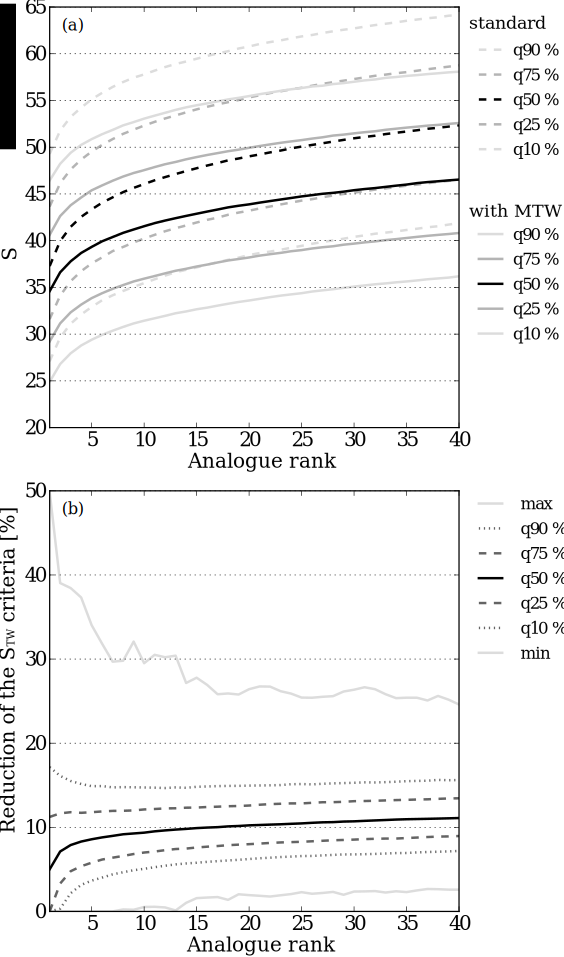
\includegraphics[width=8.2cm]{figures/changes_S1_value_and_gain.pdf}
%DIFDELCMD < 	%%%
\DIFdelendFL \DIFaddbeginFL \includegraphics[width=8.2cm]{fig07.pdf}
		\DIFaddendFL \end{center}
		\caption{Synthesis of the changes in the \DIFdelbeginFL \DIFdelFL{$S_{\text{TW}}$ criteria, }\DIFdelendFL \DIFaddbeginFL \DIFaddFL{S1 criterion }\DIFaddendFL due to the MTW \DIFdelbeginFL \DIFdelFL{, }\DIFdelendFL for the Ulrichen station \DIFdelbeginFL \DIFdelFL{, }\DIFdelendFL depending on the \DIFdelbeginFL \DIFdelFL{ranks }\DIFdelendFL \DIFaddbeginFL \DIFaddFL{rank }\DIFaddendFL of the analogue. (a) Quantiles of the \DIFdelbeginFL \DIFdelFL{$S_{\text{TW}}$ }\DIFdelendFL \DIFaddbeginFL \DIFaddFL{S1 }\DIFaddendFL distributions with and without the MTW. (b) Quantiles of the relative improvements of the S1 \DIFdelbeginFL \DIFdelFL{criteria }\DIFdelendFL \DIFaddbeginFL \DIFaddFL{criterion }\DIFaddendFL when using the MTW.}
		\label{fig:changes_S1}
	\end{figure}

	\begin{figure}[htb]
		\begin{center}
			\DIFdelbeginFL %DIFDELCMD < \includegraphics[width=8.3cm]{figures/changes_S1_precip_threshold.pdf}
%DIFDELCMD < 	%%%
\DIFdelendFL \DIFaddbeginFL \includegraphics[width=8.3cm]{fig08.pdf}
		\DIFaddendFL \end{center}
		\caption{Distribution of the median improvements of the \DIFdelbeginFL \DIFdelFL{$S_{\text{TW}}$ criteria, }\DIFdelendFL \DIFaddbeginFL \DIFaddFL{S1 criterion }\DIFaddendFL due to the MTW \DIFdelbeginFL \DIFdelFL{, }\DIFdelendFL depending on \DIFaddbeginFL \DIFaddFL{daily }\DIFaddendFL precipitation thresholds at the Ulrichen station.}
		\label{fig:changes_S1_precip_threshold}
	\end{figure}

	\begin{figure}[htb]
		\begin{center}
			\DIFdelbeginFL %DIFDELCMD < 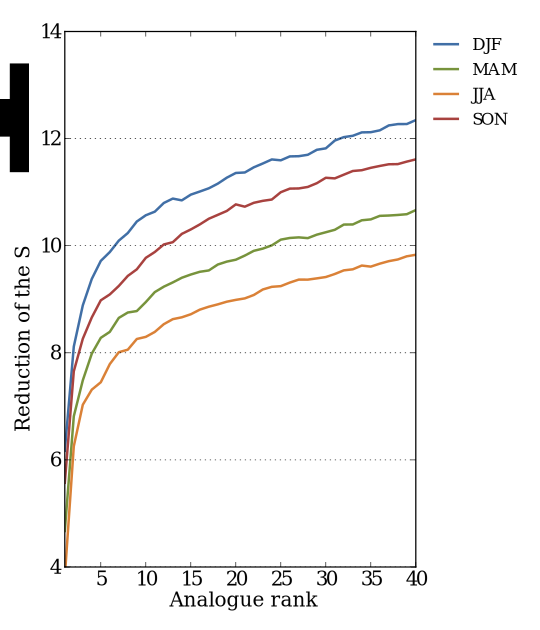
\includegraphics[width=7cm]{figures/changes_S1_seasons.pdf}
%DIFDELCMD < 	%%%
\DIFdelendFL \DIFaddbeginFL \includegraphics[width=7cm]{fig09.pdf}
		\DIFaddendFL \end{center}
		\caption{Seasonal effect on the median reduction of the \DIFdelbeginFL \DIFdelFL{$S_{\text{TW}}$ criteria }\DIFdelendFL \DIFaddbeginFL \DIFaddFL{S1 criterion }\DIFaddendFL for the Ulrichen station due to the MTW. DJF: winter, MAM: spring, JJA: summer\DIFaddbeginFL \DIFaddFL{, and }\DIFaddendFL SON: fall.}
		\label{fig:changes_S1_seasons}
	\end{figure}

	\begin{figure}[htb]
		\DIFdelbeginFL %DIFDELCMD < \includegraphics[width=8.3cm]{figures/hours_selection_per_season.pdf}
%DIFDELCMD < 	%%%
%DIFDELCMD < \caption{%
{%DIFAUXCMD
\DIFdelFL{Distribution of the predictors hours in the selected analogue dates depending on the season, for the Ulrichen station.}}
	%DIFAUXCMD
%DIFDELCMD < \label{fig:hours_selection_per_season}
%DIFDELCMD < \end{figure}
%DIFDELCMD < 

%DIFDELCMD < \begin{figure}[htb]
%DIFDELCMD < 	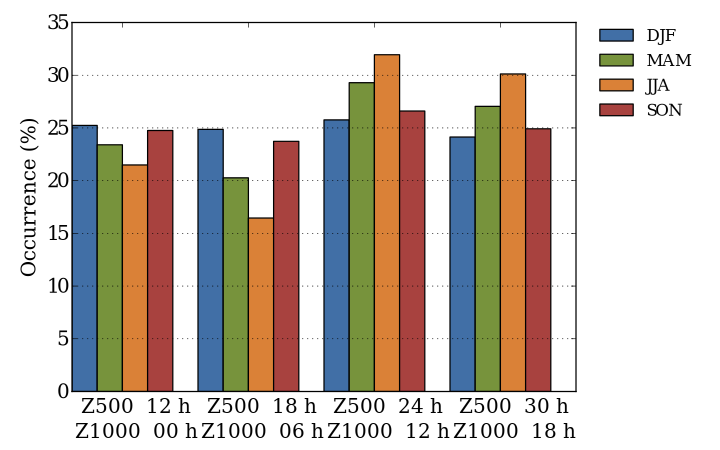
\includegraphics[width=8.3cm]{figures/hours_selection_per_season_Visp.pdf}
%DIFDELCMD < 	%%%
%DIFDELCMD < \caption{%
{%DIFAUXCMD
\DIFdelFL{Distribution of the predictors hours in the selected analogue dates depending on the season, for the Visp station.}}
	%DIFAUXCMD
%DIFDELCMD < \label{fig:hours_selection_per_season_Visp}
%DIFDELCMD < \end{figure}
%DIFDELCMD < 

%DIFDELCMD < \begin{figure}[htb]
%DIFDELCMD < 	%%%
\DIFdelendFL \begin{center}
			\DIFdelbeginFL %DIFDELCMD < 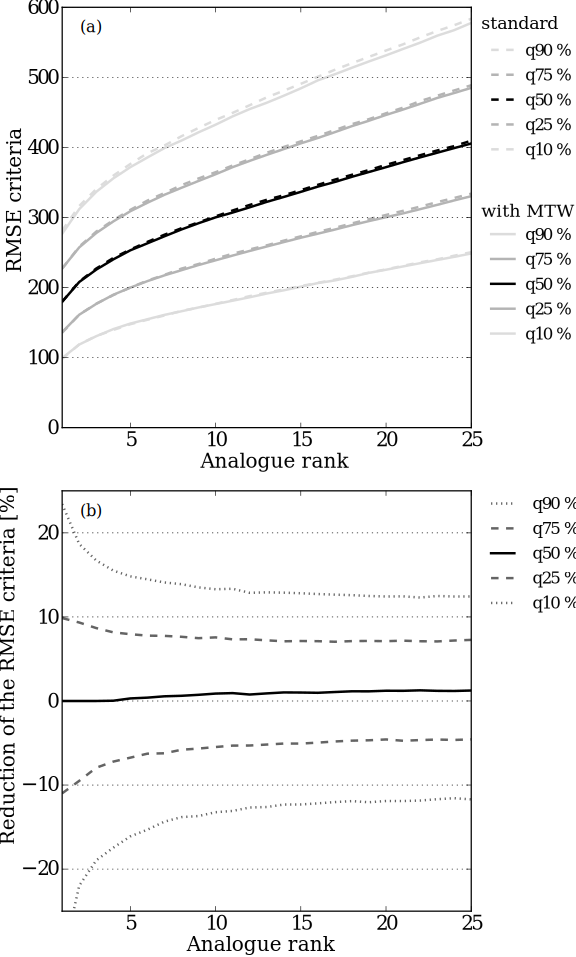
\includegraphics[width=8.1cm]{figures/changes_RMSE_value_and_gain.pdf}
%DIFDELCMD < 	%%%
\DIFdelendFL \DIFaddbeginFL \includegraphics[width=8.1cm]{fig10.pdf}
		\DIFaddendFL \end{center}
		\caption{Synthesis of the changes in the \DIFdelbeginFL \DIFdelFL{$E_{\text{RMS}}$ criteria, }\DIFdelendFL \DIFaddbeginFL \DIFaddFL{RMSE criterion }\DIFaddendFL due to the MTW \DIFdelbeginFL \DIFdelFL{, }\DIFdelendFL for the Ulrichen station \DIFdelbeginFL \DIFdelFL{, }\DIFdelendFL depending on the \DIFdelbeginFL \DIFdelFL{ranks }\DIFdelendFL \DIFaddbeginFL \DIFaddFL{rank }\DIFaddendFL of the analogue. (a) Quantiles of the \DIFdelbeginFL \DIFdelFL{$E_{\text{RMS}}$ }\DIFdelendFL \DIFaddbeginFL \DIFaddFL{RMSE }\DIFaddendFL distributions with and without the MTW. (b) Quantiles of the relative improvements of the \DIFdelbeginFL \DIFdelFL{$E_{\text{RMS}}$ criteria }\DIFdelendFL \DIFaddbeginFL \DIFaddFL{RMSE criterion }\DIFaddendFL when using the MTW.}
		\label{fig:changes_RMSE}
	\end{figure}

	\begin{figure}[htb]
		\DIFdelbeginFL %DIFDELCMD < 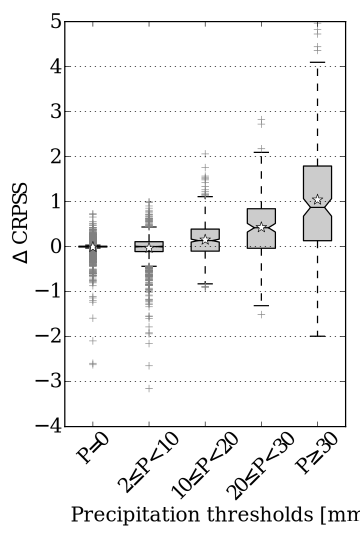
\includegraphics[width=5cm]{figures/changes_CRPS_precip_threshold.pdf}
%DIFDELCMD < 	%%%
\DIFdelendFL \DIFaddbeginFL \includegraphics[width=5cm]{fig11.pdf}
		\DIFaddendFL \caption{Differences of the \DIFdelbeginFL \DIFdelFL{$S_{\text{SCRP}}$ }\DIFdelendFL \DIFaddbeginFL \DIFaddFL{CRPSS }\DIFaddendFL performance score \DIFdelbeginFL \DIFdelFL{, }\DIFdelendFL due to the introduction of the MTW \DIFdelbeginFL \DIFdelFL{, }\DIFdelendFL as a function of \DIFaddbeginFL \DIFaddFL{daily }\DIFaddendFL precipitation thresholds at the Ulrichen station. The stars represent averages.}
		\label{fig:changes_CRPS_precip_threshold}
	\end{figure}

	\DIFdelbegin %DIFDELCMD < \begin{figure*}[htb]
%DIFDELCMD < 	\begin{center}%%%
\DIFdelFL{$
		\begin{array}{cccc}
		%\includegraphics[width=16cm]{figures/components.pdf}
		\end{array}$
	}%DIFDELCMD < \end{center}
%DIFDELCMD < 	%%%
%DIFDELCMD < \caption{%
{%DIFAUXCMD
\DIFdelFL{Influence (\%) of the MTW on the $S_{\text{CRP}}$ components (accuracy and sharpness) relatively to the total $S_{\text{CRP}}$, for the 2Z and 2Z-2MI methods, according to different precipitation thresholds. The results are presented for (top) the original parameters, and (bottom) the recalibrated parameters. Improved prediction results in a lower score.}}
	%DIFAUXCMD
%DIFDELCMD < \label{fig:CRPSS_decomposition_precip_thresholds}
%DIFDELCMD < \end{figure*}
%DIFDELCMD < 

%DIFDELCMD < %%%
\DIFdelend \begin{figure}[htb]
		\DIFdelbeginFL %DIFDELCMD < \begin{center}
%DIFDELCMD < 		\includegraphics[width=8cm]{figures/illustration_disaggregation.pdf}
%DIFDELCMD < 	\end{center}
%DIFDELCMD < 	%%%
\DIFdelendFL \DIFaddbeginFL \includegraphics[width=8.3cm]{fig12.pdf}
		\DIFaddendFL \caption{\DIFdelbeginFL \DIFdelFL{Illustration }\DIFdelendFL \DIFaddbeginFL \DIFaddFL{Distribution }\DIFaddendFL of the \DIFdelbeginFL \DIFdelFL{generation of 24~h-totals moving averages by means of a proportional distribution. The colours refer to }\DIFdelendFL \DIFaddbeginFL \DIFaddFL{predictor hours on }\DIFaddendFL the \DIFdelbeginFL \DIFdelFL{corresponding day of }\DIFdelendFL \DIFaddbeginFL \DIFaddFL{selected analogue dates, when using }\DIFaddendFL the \DIFdelbeginFL \DIFdelFL{daily time series}\DIFdelendFL \DIFaddbeginFL \DIFaddFL{MTW, depending on the season for the Ulrichen station}\DIFaddendFL .}
		\DIFdelbeginFL %DIFDELCMD < \label{fig:illustration_disaggregation}
%DIFDELCMD < %%%
\DIFdelendFL \DIFaddbeginFL \label{fig:hours_selection_per_season}
	\DIFaddendFL \end{figure}

	
	\clearpage

	
	\begin{table}[htb]
		\caption{Parameters \DIFdelbeginFL \DIFdelFL{of }\DIFdelendFL \DIFaddbeginFL \DIFaddFL{for }\DIFaddendFL the reference method on the atmospheric circulation (2Z). The first column is the level of analogy (0 for preselection), \DIFdelbeginFL \DIFdelFL{then comes }\DIFdelendFL the \DIFaddbeginFL \DIFaddFL{second column is the }\DIFaddendFL meteorological variable\DIFaddbeginFL \DIFaddFL{, }\DIFaddendFL and \DIFaddbeginFL \DIFaddFL{then }\DIFaddendFL its hour of observation (temporal window). The \DIFdelbeginFL \DIFdelFL{criteria }\DIFdelendFL \DIFaddbeginFL \DIFaddFL{criterion }\DIFaddendFL used for the current level of analogy is then provided, as well as the number of analogues.}
		\footnotesize
		\begin{center}
			\begin{tabular}{ccccc}
				\hline
				Level & Variable & Hour & \DIFdelbeginFL \DIFdelFL{Criteria }\DIFdelendFL \DIFaddbeginFL \DIFaddFL{Criterion }\DIFaddendFL & Nb \\ 
				\hline 
				0 & \multicolumn{4}{l}{$\pm 60$ days around the target date} \\
				\hline 
				\multirow{2}{*}{1} & Z1000 & 12~h & \DIFdelbeginFL %DIFDELCMD < \multirow{2}{*}{$S_{\text{TW}}$} %%%
\DIFdelendFL \DIFaddbeginFL \multirow{2}{*}{S1} \DIFaddendFL & \multirow{2}{*}{$N_{1}$} \\
				& Z500 & 24~h & & \\ 
				\hline 
			\end{tabular} 
		\end{center}
		\label{table:method_2Z}
	\end{table}

	\begin{table}[htb]
		\caption{Parameters of the reference method with moisture variables (2Z-2MI). Same conventions as Table \ref{table:method_2Z}}
		\footnotesize
		\begin{center}
			\begin{tabular}{ccccc}
				\hline 
				Level & Variable & Hour & \DIFdelbeginFL \DIFdelFL{Criteria }\DIFdelendFL \DIFaddbeginFL \DIFaddFL{Criterion }\DIFaddendFL & Nb \\ 
				\hline 
				0 & \multicolumn{4}{l}{$\pm 60$ days around the target date} \\
				\hline 
				\multirow{2}{*}{1} & Z1000 & 12~h & \DIFdelbeginFL %DIFDELCMD < \multirow{2}{*}{$S_{\text{TW}}$} %%%
\DIFdelendFL \DIFaddbeginFL \multirow{2}{*}{S1} \DIFaddendFL & \multirow{2}{*}{$N_{1}$} \\
				& Z500 & 24~h & & \\ 
				\hline
				\multirow{2}{*}{2} & TPW * RH850 & 12~h & \DIFdelbeginFL %DIFDELCMD < \multirow{2}{*}{$E_{\text{RMS}}$} %%%
\DIFdelendFL \DIFaddbeginFL \multirow{2}{*}{RMSE} \DIFaddendFL & \multirow{2}{*}{$N_{2}$} \\
				& TPW * RH850 & 24~h & & \\ 
				\hline 
			\end{tabular} 
		\end{center}
		\label{table:method_2Z-2MI}
	\end{table}

	\begin{table}[htb]
		\caption{\DIFdelbeginFL \DIFdelFL{Calibrated parameters (spatial windows and }\DIFdelendFL \DIFaddbeginFL \DIFaddFL{Optimal }\DIFaddendFL number of analogues \DIFdelbeginFL \DIFdelFL{) for }\DIFdelendFL \DIFaddbeginFL \DIFaddFL{(of }\DIFaddendFL the \DIFaddbeginFL \DIFaddFL{first and second level of }\DIFaddendFL analogy\DIFaddbeginFL \DIFaddFL{, respectively, $N_{1}$ and $N_{2}$) of the method based }\DIFaddendFL on the \DIFdelbeginFL \DIFdelFL{geopotential at 500~hPa and 1000~hPa }\DIFdelendFL \DIFaddbeginFL \DIFaddFL{atmospheric circulation only }\DIFaddendFL (method 2Z) and \DIFdelbeginFL \DIFdelFL{skill score (\%) of }\DIFdelendFL the method \DIFaddbeginFL \DIFaddFL{with a second level of analogy with moisture variables (2Z-2MI) }\DIFaddendFL on the full archive \DIFaddbeginFL \DIFaddFL{(Standard), and after recalibration using the MTW (MTW-r)}\DIFaddendFL .}
		\begin{center}
			\DIFdelbeginFL %DIFDELCMD < \begin{tabular}{l c c c c }
%DIFDELCMD < 			%%%
\DIFdelendFL \DIFaddbeginFL \begin{tabular}{l c c c c c c }
				\DIFaddendFL \hline
				\DIFdelbeginFL \DIFdelFL{Station }\DIFdelendFL \DIFaddbeginFL \multirow{3}{*}{Station} \DIFaddendFL & \DIFdelbeginFL \DIFdelFL{Long (° E) }\DIFdelendFL \DIFaddbeginFL \multicolumn{3}{c}{Standard} \DIFaddendFL & \DIFdelbeginFL \DIFdelFL{Lat (° N) }%DIFDELCMD < & %%%
\DIFdelFL{$N_{1}$ }%DIFDELCMD < & %%%
\DIFdelFL{$S_{\text{SCRP}}$ }\DIFdelendFL \DIFaddbeginFL \multicolumn{3}{c}{MTW-r} \DIFaddendFL \\
				\DIFdelbeginFL %DIFDELCMD < \hline
%DIFDELCMD < 			%%%
\DIFdelFL{Ulrichen }\DIFdelendFL & \DIFdelbeginFL \DIFdelFL{0 $\rightarrow$ 17.5 }\DIFdelendFL \DIFaddbeginFL \DIFaddFL{2Z }\DIFaddendFL & \DIFdelbeginFL \DIFdelFL{42.5 $\rightarrow$ 47.5 }\DIFdelendFL \DIFaddbeginFL \multicolumn{2}{c}{2Z-2MI} \DIFaddendFL & \DIFdelbeginFL \DIFdelFL{40 }\DIFdelendFL \DIFaddbeginFL \DIFaddFL{2Z }\DIFaddendFL & \DIFdelbeginFL \DIFdelFL{30.73 }\DIFdelendFL \DIFaddbeginFL \multicolumn{2}{c}{2Z-2MI}\DIFaddendFL \\
				\DIFdelbeginFL \DIFdelFL{Zermatt }\DIFdelendFL & \DIFdelbeginFL \DIFdelFL{0 $\rightarrow$ 20 }\DIFdelendFL \DIFaddbeginFL \DIFaddFL{$N_{1}$ }\DIFaddendFL & \DIFdelbeginFL \DIFdelFL{37.5 $\rightarrow$ 50 }\DIFdelendFL \DIFaddbeginFL \DIFaddFL{$N_{1}$ }\DIFaddendFL & \DIFdelbeginFL \DIFdelFL{35 }\DIFdelendFL \DIFaddbeginFL \DIFaddFL{$N_{2}$ }\DIFaddendFL & \DIFdelbeginFL \DIFdelFL{23.87 }%DIFDELCMD < \\
%DIFDELCMD < 			%%%
\DIFdelFL{Visp }\DIFdelendFL \DIFaddbeginFL \DIFaddFL{$N_{1}$ }\DIFaddendFL & \DIFdelbeginFL \DIFdelFL{-2.5 $\rightarrow$ 20 }%DIFDELCMD < & %%%
\DIFdelFL{40 $\rightarrow$ 47.5 }%DIFDELCMD < & %%%
\DIFdelFL{30 }%DIFDELCMD < & %%%
\DIFdelFL{25.11 }%DIFDELCMD < \\
%DIFDELCMD < 			%%%
\DIFdelFL{Montana }%DIFDELCMD < & %%%
\DIFdelFL{-2.5 $\rightarrow$ 17.5 }%DIFDELCMD < & %%%
\DIFdelFL{40 $\rightarrow$ 47.5 }%DIFDELCMD < & %%%
\DIFdelFL{40 }%DIFDELCMD < & %%%
\DIFdelFL{32.55 }%DIFDELCMD < \\
%DIFDELCMD < 			%%%
\DIFdelFL{Sion }%DIFDELCMD < & %%%
\DIFdelFL{-2.5 $\rightarrow$ 17.5 }%DIFDELCMD < & %%%
\DIFdelFL{40 $\rightarrow$ 47.5 }%DIFDELCMD < & %%%
\DIFdelFL{40 }%DIFDELCMD < & %%%
\DIFdelFL{26.23 }%DIFDELCMD < \\
%DIFDELCMD < 			%%%
\DIFdelFL{Aigle }%DIFDELCMD < & %%%
\DIFdelFL{-5 $\rightarrow$ 17.5 }%DIFDELCMD < & %%%
\DIFdelFL{40 $\rightarrow$ 50 }%DIFDELCMD < & %%%
\DIFdelFL{50 }%DIFDELCMD < & %%%
\DIFdelFL{30.59 }%DIFDELCMD < \\ 
%DIFDELCMD < 			\hline
%DIFDELCMD < 		\end{tabular}
%DIFDELCMD < 	\end{center}
%DIFDELCMD < 	\label{table:params_2Z}
%DIFDELCMD < \end{table}
%DIFDELCMD < 

%DIFDELCMD < \begin{table}[htb]
%DIFDELCMD < 	%%%
%DIFDELCMD < \caption{%
{%DIFAUXCMD
\DIFdelFL{Parameters of the moisture variables from the 2Z-2MI method and the corresponding skill score (\%) on the complete archive. The parameters for the atmospheric circulation are the same as in Table \ref{table:params_2Z}, except the number of analogues of the first analogy level ($N_{1}$), which are here different. The $5^{th}$ column is the number of analogues for the second level ($N_{2}$).}}
	%DIFAUXCMD
%DIFDELCMD < \begin{center}
%DIFDELCMD < 		\begin{tabular}{l c c c c c }
%DIFDELCMD < 			\hline
%DIFDELCMD < 			%%%
\DIFdelFL{Station }%DIFDELCMD < & %%%
\DIFdelFL{Long (° E) }%DIFDELCMD < & %%%
\DIFdelFL{Lat (° N) }%DIFDELCMD < & %%%
\DIFdelendFL $N_{1}$ & $N_{2}$\DIFdelbeginFL %DIFDELCMD < & %%%
\DIFdelFL{$S_{\text{SCRP}}$ }\DIFdelendFL \\ 
				\hline
				Ulrichen & \DIFdelbeginFL \DIFdelFL{5 $\rightarrow$ 10 }\DIFdelendFL \DIFaddbeginFL \DIFaddFL{40 }\DIFaddendFL & \DIFdelbeginFL \DIFdelFL{45 $\rightarrow$ 47.5 }%DIFDELCMD < & %%%
\DIFdelendFL 60 & 25 & \DIFdelbeginFL \DIFdelFL{34.31 }\DIFdelendFL \DIFaddbeginFL \DIFaddFL{50 }& \DIFaddFL{110 }& \DIFaddFL{35}\DIFaddendFL \\
				Zermatt & \DIFdelbeginFL \DIFdelFL{5 $\rightarrow$ 10 }\DIFdelendFL \DIFaddbeginFL \DIFaddFL{35 }\DIFaddendFL & \DIFdelbeginFL \DIFdelFL{45 $\rightarrow$ 47.5 }%DIFDELCMD < & %%%
\DIFdelendFL 55 & 25 & \DIFdelbeginFL \DIFdelFL{28.28 }\DIFdelendFL \DIFaddbeginFL \DIFaddFL{55 }& \DIFaddFL{80 }& \DIFaddFL{30}\DIFaddendFL \\
				Visp & \DIFdelbeginFL \DIFdelFL{5 $\rightarrow$ 10 }\DIFdelendFL \DIFaddbeginFL \DIFaddFL{30 }\DIFaddendFL & 45 \DIFdelbeginFL \DIFdelFL{$\rightarrow$ 47.5 }\DIFdelendFL & \DIFdelbeginFL \DIFdelFL{45 }%DIFDELCMD < & %%%
\DIFdelendFL 25 & \DIFdelbeginFL \DIFdelFL{28.85 }%DIFDELCMD < \\
%DIFDELCMD < 			%%%
\DIFdelFL{Montana }%DIFDELCMD < & %%%
\DIFdelFL{5 $\rightarrow$ 7.5 }%DIFDELCMD < & %%%
\DIFdelFL{45 $\rightarrow$ 47.5 }%DIFDELCMD < & %%%
\DIFdelendFL 55 & \DIFdelbeginFL \DIFdelFL{30 }\DIFdelendFL \DIFaddbeginFL \DIFaddFL{135 }\DIFaddendFL & \DIFdelbeginFL \DIFdelFL{36.11 }%DIFDELCMD < \\
%DIFDELCMD < 			%%%
\DIFdelFL{Sion }%DIFDELCMD < & %%%
\DIFdelFL{5 $\rightarrow$ 10 }%DIFDELCMD < & %%%
\DIFdelFL{45 $\rightarrow$ 47.5 }%DIFDELCMD < & %%%
\DIFdelFL{90 }%DIFDELCMD < & %%%
\DIFdelFL{30 }%DIFDELCMD < & %%%
\DIFdelFL{31.16 }%DIFDELCMD < \\
%DIFDELCMD < 			%%%
\DIFdelFL{Aigle }%DIFDELCMD < & %%%
\DIFdelFL{7.5 }%DIFDELCMD < & %%%
\DIFdelFL{45 $\rightarrow$ 47.5 }%DIFDELCMD < & %%%
\DIFdelFL{100 }%DIFDELCMD < & %%%
\DIFdelendFL 35\DIFdelbeginFL %DIFDELCMD < & %%%
\DIFdelFL{35.82 }\DIFdelendFL \\
				\DIFdelbeginFL %DIFDELCMD < \hline
%DIFDELCMD < 		\end{tabular}
%DIFDELCMD < 	\end{center}
%DIFDELCMD < 	\label{table:params_2Z-2MI}
%DIFDELCMD < \end{table}
%DIFDELCMD < 

%DIFDELCMD < \begin{table}[htb]
%DIFDELCMD < 	%%%
%DIFDELCMD < \caption{%
{%DIFAUXCMD
\DIFdelFL{Influence of the archive reduction on the $S_{\text{SCRP}}$. $S_{\text{SCRP}}$ values are provided for both considered methods and the differences are expressed in absolute value.}}
	%DIFAUXCMD
%DIFDELCMD < \begin{center}
%DIFDELCMD < 		\begin{tabular}{l c c c c }
%DIFDELCMD < 			\hline
%DIFDELCMD < 			\multirow{2}{*}{Station} & \multicolumn{2}{c}{2Z} & \multicolumn{2}{c}{2Z-2MI} \\
%DIFDELCMD < 			& %%%
\DIFdelFL{82-07 }%DIFDELCMD < & %%%
\DIFdelFL{$\Delta$ }%DIFDELCMD < & %%%
\DIFdelFL{82-07 }%DIFDELCMD < & %%%
\DIFdelFL{$\Delta$ }%DIFDELCMD < \\ 
%DIFDELCMD < 			\hline
%DIFDELCMD < 			%%%
\DIFdelFL{Ulrichen }%DIFDELCMD < & %%%
\DIFdelFL{29.37 }%DIFDELCMD < & %%%
\DIFdelFL{-1.36 }%DIFDELCMD < & %%%
\DIFdelFL{33.24 }%DIFDELCMD < & %%%
\DIFdelFL{-1.08 }%DIFDELCMD < \\
%DIFDELCMD < 			%%%
\DIFdelFL{Zermatt }%DIFDELCMD < & %%%
\DIFdelFL{22.20 }%DIFDELCMD < & %%%
\DIFdelFL{-1.67 }%DIFDELCMD < & %%%
\DIFdelFL{26.95 }%DIFDELCMD < & %%%
\DIFdelFL{-1.32 }%DIFDELCMD < \\
%DIFDELCMD < 			%%%
\DIFdelFL{Visp }%DIFDELCMD < & %%%
\DIFdelFL{23.23 }%DIFDELCMD < & %%%
\DIFdelFL{-1.89 }%DIFDELCMD < & %%%
\DIFdelFL{27.77 }%DIFDELCMD < & %%%
\DIFdelFL{-1.08 }%DIFDELCMD < \\
%DIFDELCMD < 			%%%
\DIFdelendFL Montana & \DIFdelbeginFL \DIFdelFL{30.79 }\DIFdelendFL \DIFaddbeginFL \DIFaddFL{40 }\DIFaddendFL & \DIFdelbeginFL \DIFdelFL{-1.76 }\DIFdelendFL \DIFaddbeginFL \DIFaddFL{55 }\DIFaddendFL & \DIFdelbeginFL \DIFdelFL{34.77 }\DIFdelendFL \DIFaddbeginFL \DIFaddFL{30 }\DIFaddendFL & \DIFdelbeginFL \DIFdelFL{-1.34 }%DIFDELCMD < \\
%DIFDELCMD < 			%%%
\DIFdelFL{Sion }\DIFdelendFL \DIFaddbeginFL \DIFaddFL{55 }\DIFaddendFL & \DIFdelbeginFL \DIFdelFL{24.78 }\DIFdelendFL \DIFaddbeginFL \DIFaddFL{110 }\DIFaddendFL & \DIFdelbeginFL \DIFdelFL{-1.45 }%DIFDELCMD < & %%%
\DIFdelFL{29.36 }%DIFDELCMD < & %%%
\DIFdelFL{-1.80 }\DIFdelendFL \DIFaddbeginFL \DIFaddFL{40}\DIFaddendFL \\
				\DIFdelbeginFL \DIFdelFL{Aigle }%DIFDELCMD < & %%%
\DIFdelFL{30.57 }%DIFDELCMD < & %%%
\DIFdelFL{-0.01 }%DIFDELCMD < & %%%
\DIFdelFL{35.95 }%DIFDELCMD < & %%%
\DIFdelFL{0.13 }%DIFDELCMD < \\ 
%DIFDELCMD < 			\hline
%DIFDELCMD < 		\end{tabular}
%DIFDELCMD < 	\end{center}
%DIFDELCMD < 	\label{table:loss_reduction}
%DIFDELCMD < \end{table}
%DIFDELCMD < 

%DIFDELCMD < \begin{table}[htb]
%DIFDELCMD < 	%%%
%DIFDELCMD < \caption{%
{%DIFAUXCMD
\DIFdelFL{New $S_{\text{SCRP}}$ performance scores for both 2Z and 2Z-2MI methods obtained by the MTW approach. The differences are expressed regarding the conventional method with the same archive length.}}
	%DIFAUXCMD
%DIFDELCMD < \begin{center}
%DIFDELCMD < 		\begin{tabular}{l c c c c}
%DIFDELCMD < 			\hline
%DIFDELCMD < 			\multirow{2}{*}{Station} & \multicolumn{2}{c}{2Z} & \multicolumn{ 2}{c}{2Z-2MI} \\
%DIFDELCMD < 			& %%%
\DIFdelFL{MTW }%DIFDELCMD < & %%%
\DIFdelFL{$\Delta$ }%DIFDELCMD < & %%%
\DIFdelFL{MTW }%DIFDELCMD < & %%%
\DIFdelFL{$\Delta$ }%DIFDELCMD < \\
%DIFDELCMD < 			\hline
%DIFDELCMD < 			%%%
\DIFdelFL{Ulrichen }%DIFDELCMD < & %%%
\DIFdelFL{31.12 }%DIFDELCMD < & %%%
\DIFdelFL{1.74 }%DIFDELCMD < & %%%
\DIFdelFL{35.44 }%DIFDELCMD < & %%%
\DIFdelFL{2.20 }%DIFDELCMD < \\
%DIFDELCMD < 			%%%
\DIFdelFL{Zermatt }%DIFDELCMD < & %%%
\DIFdelFL{24.34 }%DIFDELCMD < & %%%
\DIFdelFL{2.14 }%DIFDELCMD < & %%%
\DIFdelFL{28.92 }%DIFDELCMD < & %%%
\DIFdelFL{1.97 }%DIFDELCMD < \\
%DIFDELCMD < 			%%%
\DIFdelFL{Visp }%DIFDELCMD < & %%%
\DIFdelFL{24.39 }%DIFDELCMD < & %%%
\DIFdelFL{1.16 }%DIFDELCMD < & %%%
\DIFdelFL{29.42 }%DIFDELCMD < & %%%
\DIFdelFL{1.64 }%DIFDELCMD < \\
%DIFDELCMD < 			%%%
\DIFdelFL{Montana }%DIFDELCMD < & %%%
\DIFdelFL{31.59 }%DIFDELCMD < & %%%
\DIFdelFL{0.80 }%DIFDELCMD < & %%%
\DIFdelFL{36.30 }%DIFDELCMD < & %%%
\DIFdelFL{1.53 }%DIFDELCMD < \\
%DIFDELCMD < 			%%%
\DIFdelendFL Sion & \DIFdelbeginFL \DIFdelFL{25.35 }%DIFDELCMD < & %%%
\DIFdelFL{0.57 }%DIFDELCMD < & %%%
\DIFdelFL{31.07 }%DIFDELCMD < & %%%
\DIFdelFL{1.71 }%DIFDELCMD < \\
%DIFDELCMD < 			%%%
\DIFdelFL{Aigle }%DIFDELCMD < & %%%
\DIFdelFL{31.78 }%DIFDELCMD < & %%%
\DIFdelFL{1.21 }%DIFDELCMD < & %%%
\DIFdelFL{38.11 }%DIFDELCMD < & %%%
\DIFdelFL{2.16 }%DIFDELCMD < \\ 
%DIFDELCMD < 			\hline
%DIFDELCMD < 		\end{tabular}
%DIFDELCMD < 	\end{center}
%DIFDELCMD < 	\label{table:CRPSS_MTW}
%DIFDELCMD < \end{table}
%DIFDELCMD < 

%DIFDELCMD < \begin{table}[htb]
%DIFDELCMD < 	%%%
%DIFDELCMD < \caption{%
{%DIFAUXCMD
\DIFdelFL{Calibrated parameters (spatial windows and number of analogues) for the analogy on the geopotential at 500~hPa and 1000~hPa (method 2Z) with the MTW approach.}}
	%DIFAUXCMD
%DIFDELCMD < \begin{center}
%DIFDELCMD < 		\begin{tabular}{l c c c }
%DIFDELCMD < 			\hline
%DIFDELCMD < 			%%%
\DIFdelFL{Station }%DIFDELCMD < & %%%
\DIFdelFL{Long (° E) }%DIFDELCMD < & %%%
\DIFdelFL{Lat (° N) }%DIFDELCMD < & %%%
\DIFdelFL{$N_{1}$ }%DIFDELCMD < \\
%DIFDELCMD < 			\hline
%DIFDELCMD < 			%%%
\DIFdelFL{Ulrichen }%DIFDELCMD < & %%%
\DIFdelFL{0 $\rightarrow$ 17.5 }%DIFDELCMD < & %%%
\DIFdelFL{42.5 $\rightarrow$ 50 }%DIFDELCMD < & %%%
\DIFdelFL{50 }%DIFDELCMD < \\
%DIFDELCMD < 			%%%
\DIFdelFL{Zermatt }%DIFDELCMD < & %%%
\DIFdelFL{0 $\rightarrow$ 17.5 }%DIFDELCMD < & %%%
\DIFdelendFL 40 \DIFdelbeginFL \DIFdelFL{$\rightarrow$ 50 }\DIFdelendFL & \DIFdelbeginFL \DIFdelFL{55 }%DIFDELCMD < \\
%DIFDELCMD < 			%%%
\DIFdelFL{Visp }\DIFdelendFL \DIFaddbeginFL \DIFaddFL{90 }\DIFaddendFL & \DIFdelbeginFL \DIFdelFL{-2.5 $\rightarrow$ 20 }\DIFdelendFL \DIFaddbeginFL \DIFaddFL{30 }\DIFaddendFL & \DIFdelbeginFL \DIFdelFL{40 $\rightarrow$ 50 }%DIFDELCMD < & %%%
\DIFdelendFL 55 \DIFdelbeginFL %DIFDELCMD < \\
%DIFDELCMD < 			%%%
\DIFdelFL{Montana }\DIFdelendFL & \DIFdelbeginFL \DIFdelFL{-2.5 $\rightarrow$ 15 }\DIFdelendFL \DIFaddbeginFL \DIFaddFL{140 }\DIFaddendFL & \DIFdelbeginFL \DIFdelFL{42.5 $\rightarrow$ 47.5 }%DIFDELCMD < & %%%
\DIFdelFL{55 }%DIFDELCMD < \\
%DIFDELCMD < 			%%%
\DIFdelFL{Sion }%DIFDELCMD < & %%%
\DIFdelFL{-2.5 $\rightarrow$ 15 }%DIFDELCMD < & %%%
\DIFdelFL{37.5 $\rightarrow$ }\DIFdelendFL 50\DIFdelbeginFL %DIFDELCMD < & %%%
\DIFdelFL{55 }\DIFdelendFL \\
				Aigle & \DIFdelbeginFL \DIFdelFL{-2.5 $\rightarrow$ 15 }%DIFDELCMD < & %%%
\DIFdelFL{40 $\rightarrow$ }\DIFdelendFL 50 & \DIFdelbeginFL \DIFdelFL{75 }%DIFDELCMD < \\
%DIFDELCMD < 			\hline
%DIFDELCMD < 		\end{tabular}
%DIFDELCMD < 	\end{center}
%DIFDELCMD < 	\label{table:params_2Z_new}
%DIFDELCMD < \end{table}
%DIFDELCMD < 

%DIFDELCMD < \begin{table}[htb]
%DIFDELCMD < 	%%%
%DIFDELCMD < \caption{%
{%DIFAUXCMD
\DIFdelFL{Parameters of the moisture variables from the 2Z-2MI method with the MTW approach. The parameters for the atmospheric circulation are the same as in Table \ref{table:params_2Z_new}, except the number of analogues of the first analogy level ($N_{1}$), which are here different. The $5^{th}$ column is the number of analogues for the second level ($N_{2}$).}}
	%DIFAUXCMD
%DIFDELCMD < \begin{center}
%DIFDELCMD < 		\begin{tabular}{l c c c c }
%DIFDELCMD < 			\hline
%DIFDELCMD < 			%%%
\DIFdelFL{Station }\DIFdelendFL \DIFaddbeginFL \DIFaddFL{100 }\DIFaddendFL & \DIFdelbeginFL \DIFdelFL{Long (° E) }%DIFDELCMD < & %%%
\DIFdelFL{Lat (° N) }%DIFDELCMD < & %%%
\DIFdelFL{$N_{1}$ }%DIFDELCMD < & %%%
\DIFdelFL{$N_{2}$ }%DIFDELCMD < \\
%DIFDELCMD < 			\hline
%DIFDELCMD < 			%%%
\DIFdelFL{Ulrichen }%DIFDELCMD < & %%%
\DIFdelFL{5 $\rightarrow$ 10 }%DIFDELCMD < & %%%
\DIFdelFL{45 $\rightarrow$ 47.5 }%DIFDELCMD < & %%%
\DIFdelFL{110 }%DIFDELCMD < & %%%
\DIFdelendFL 35 \DIFdelbeginFL %DIFDELCMD < \\
%DIFDELCMD < 			%%%
\DIFdelFL{Zermatt }\DIFdelendFL & \DIFdelbeginFL \DIFdelFL{7.5 }\DIFdelendFL \DIFaddbeginFL \DIFaddFL{75 }\DIFaddendFL & \DIFdelbeginFL \DIFdelFL{45 $\rightarrow$ 47.5 }%DIFDELCMD < & %%%
\DIFdelFL{80 }%DIFDELCMD < & %%%
\DIFdelFL{30 }%DIFDELCMD < \\
%DIFDELCMD < 			%%%
\DIFdelFL{Visp }%DIFDELCMD < & %%%
\DIFdelFL{7.5 }%DIFDELCMD < & %%%
\DIFdelFL{45 $\rightarrow$ 47.5 }%DIFDELCMD < & %%%
\DIFdelendFL 135 & \DIFdelbeginFL \DIFdelFL{35 }%DIFDELCMD < \\
%DIFDELCMD < 			%%%
\DIFdelFL{Montana }%DIFDELCMD < & %%%
\DIFdelFL{5 $\rightarrow$ 7.5 }%DIFDELCMD < & %%%
\DIFdelendFL 45\DIFdelbeginFL %DIFDELCMD < & %%%
\DIFdelFL{110 }%DIFDELCMD < & %%%
\DIFdelFL{40 }\DIFdelendFL \\ 
				\DIFdelbeginFL \DIFdelFL{Sion }%DIFDELCMD < & %%%
\DIFdelFL{5 $\rightarrow$ 10 }%DIFDELCMD < & %%%
\DIFdelFL{45 $\rightarrow$ 47.5 }%DIFDELCMD < & %%%
\DIFdelFL{140 }%DIFDELCMD < & %%%
\DIFdelFL{50 }%DIFDELCMD < \\
%DIFDELCMD < 			%%%
\DIFdelFL{Aigle }%DIFDELCMD < & %%%
\DIFdelFL{5 $\rightarrow$ 7.5 }%DIFDELCMD < & %%%
\DIFdelFL{45 }%DIFDELCMD < & %%%
\DIFdelFL{135 }%DIFDELCMD < & %%%
\DIFdelFL{45 }%DIFDELCMD < \\ 
%DIFDELCMD < 			%%%
\DIFdelendFL \hline
			\end{tabular}
		\end{center}	
		\DIFdelbeginFL %DIFDELCMD < \label{table:params_2Z-2MI_new}
%DIFDELCMD < %%%
\DIFdelendFL \DIFaddbeginFL \label{table:analog_nb}
	\DIFaddendFL \end{table}

	\begin{table}[htb]
		\caption{Values of the \DIFdelbeginFL \DIFdelFL{$S_{\text{SCRP}}$ }\DIFdelendFL \DIFaddbeginFL \DIFaddFL{CRPSS }\DIFaddendFL (\%) \DIFdelbeginFL \DIFdelFL{skill }\DIFdelendFL score for the \DIFdelbeginFL \DIFdelFL{newly calibrated }\DIFdelendFL \DIFaddbeginFL \DIFaddFL{original and the recalibrated }\DIFaddendFL parameters \DIFaddbeginFL \DIFaddFL{(with the sequential method, as described in Sect. \ref{sec:calibration}) }\DIFaddendFL using the MTW approach \DIFdelbeginFL \DIFdelFL{. The differences are expressed regarding }\DIFdelendFL \DIFaddbeginFL \DIFaddFL{on }\DIFaddendFL the \DIFdelbeginFL \DIFdelFL{conventional method with }\DIFdelendFL \DIFaddbeginFL \DIFaddFL{disaggregated precipitation time series (short period) by means of }\DIFaddendFL the \DIFdelbeginFL \DIFdelFL{same archive length}\DIFdelendFL \DIFaddbeginFL \DIFaddFL{proportional distribution}\DIFaddendFL .}
		\begin{center}
			\begin{tabular}{l c c c c}
				\hline
				\multirow{2}{*}{Station} & \multicolumn{2}{c}{2Z} & \multicolumn{ 2}{c}{2Z-2MI} \\
				& \DIFdelbeginFL \DIFdelFL{MTW }%DIFDELCMD < & %%%
\DIFdelFL{$\Delta$ }%DIFDELCMD < & %%%
\DIFdelFL{MTW }%DIFDELCMD < & %%%
\DIFdelFL{$\Delta$ }%DIFDELCMD < \\
%DIFDELCMD < 			\hline
%DIFDELCMD < 			%%%
\DIFdelFL{Ulrichen }%DIFDELCMD < & %%%
\DIFdelFL{31.58 }%DIFDELCMD < & %%%
\DIFdelFL{2.20 }%DIFDELCMD < & %%%
\DIFdelFL{35.72 }%DIFDELCMD < & %%%
\DIFdelFL{2.48  }%DIFDELCMD < \\
%DIFDELCMD < 			%%%
\DIFdelFL{Zermatt }%DIFDELCMD < & %%%
\DIFdelFL{24.71 }%DIFDELCMD < & %%%
\DIFdelFL{2.51 }%DIFDELCMD < & %%%
\DIFdelFL{29.63 }%DIFDELCMD < & %%%
\DIFdelFL{2.68 }%DIFDELCMD < \\
%DIFDELCMD < 			%%%
\DIFdelFL{Visp }%DIFDELCMD < & %%%
\DIFdelFL{25.08 }%DIFDELCMD < & %%%
\DIFdelFL{1.85 }%DIFDELCMD < & %%%
\DIFdelFL{30.29 }%DIFDELCMD < & %%%
\DIFdelFL{2.52 }%DIFDELCMD < \\
%DIFDELCMD < 			%%%
\DIFdelFL{Montana }%DIFDELCMD < & %%%
\DIFdelFL{32.22 }%DIFDELCMD < & %%%
\DIFdelFL{1.43 }%DIFDELCMD < & %%%
\DIFdelFL{37.15 }%DIFDELCMD < & %%%
\DIFdelFL{2.38 }%DIFDELCMD < \\
%DIFDELCMD < 			%%%
\DIFdelFL{Sion }%DIFDELCMD < & %%%
\DIFdelFL{26.07 }%DIFDELCMD < & %%%
\DIFdelFL{1.29 }%DIFDELCMD < & %%%
\DIFdelFL{31.68 }%DIFDELCMD < & %%%
\DIFdelFL{2.32 }%DIFDELCMD < \\
%DIFDELCMD < 			%%%
\DIFdelFL{Aigle }%DIFDELCMD < & %%%
\DIFdelFL{32.21 }%DIFDELCMD < & %%%
\DIFdelFL{1.64 }%DIFDELCMD < & %%%
\DIFdelFL{38.50 }%DIFDELCMD < & %%%
\DIFdelFL{2.55 }%DIFDELCMD < \\
%DIFDELCMD < 			\hline
%DIFDELCMD < 		\end{tabular}
%DIFDELCMD < 	\end{center}
%DIFDELCMD < 	\label{table:CRPSS_recalibration}
%DIFDELCMD < \end{table}
%DIFDELCMD < 

%DIFDELCMD < \begin{table}[htb]
%DIFDELCMD < 	%%%
%DIFDELCMD < \caption{%
{%DIFAUXCMD
\DIFdelFL{Changes in sharpness and accuracy relatively to the total $S_{\text{CRP}}$, due to the introduction of the MTW. The changes are presented for both 2Z and 2Z-2MI methods with the original parameters. A decrease of the score is desirable.}}
	%DIFAUXCMD
%DIFDELCMD < \begin{center}
%DIFDELCMD < 		\begin{tabular}{l c c c c}
%DIFDELCMD < 			\hline
%DIFDELCMD < 			\multirow{2}{*}{Station} & \multicolumn{2}{c}{2Z} & \multicolumn{2}{c}{2Z-2MI} \\
%DIFDELCMD < 			& %%%
\DIFdelFL{Sharpness }%DIFDELCMD < & %%%
\DIFdelFL{Accuracy }%DIFDELCMD < & %%%
\DIFdelFL{Sharpness }%DIFDELCMD < & %%%
\DIFdelFL{Accuracy }%DIFDELCMD < \\
%DIFDELCMD < 			\hline
%DIFDELCMD < 			%%%
\DIFdelFL{Ulrichen }%DIFDELCMD < & %%%
\DIFdelFL{2.82 }%DIFDELCMD < & %%%
\DIFdelFL{-5.29 }%DIFDELCMD < & %%%
\DIFdelFL{1.00 }%DIFDELCMD < & %%%
\DIFdelFL{-4.30 }%DIFDELCMD < \\
%DIFDELCMD < 			%%%
\DIFdelFL{Zermatt }%DIFDELCMD < & %%%
\DIFdelFL{2.26 }%DIFDELCMD < & %%%
\DIFdelFL{-5.01 }%DIFDELCMD < & %%%
\DIFdelFL{0.88 }%DIFDELCMD < & %%%
\DIFdelFL{-3.58 }%DIFDELCMD < \\
%DIFDELCMD < 			%%%
\DIFdelFL{Visp }%DIFDELCMD < & %%%
\DIFdelFL{3.66 }%DIFDELCMD < & %%%
\DIFdelFL{-5.18 }%DIFDELCMD < & %%%
\DIFdelFL{2.67 }%DIFDELCMD < & %%%
\DIFdelFL{-4.94 }%DIFDELCMD < \\
%DIFDELCMD < 			%%%
\DIFdelFL{Montana }%DIFDELCMD < & %%%
\DIFdelFL{1.62 }%DIFDELCMD < & %%%
\DIFdelFL{-2.78 }%DIFDELCMD < & %%%
\DIFdelFL{0.57 }%DIFDELCMD < & %%%
\DIFdelFL{-2.91 }%DIFDELCMD < \\
%DIFDELCMD < 			%%%
\DIFdelFL{Sion }%DIFDELCMD < & %%%
\DIFdelFL{2.02 }%DIFDELCMD < & %%%
\DIFdelFL{-2.78 }%DIFDELCMD < & %%%
\DIFdelFL{0.33 }%DIFDELCMD < & %%%
\DIFdelFL{-2.75 }%DIFDELCMD < \\
%DIFDELCMD < 			%%%
\DIFdelFL{Aigle }%DIFDELCMD < & %%%
\DIFdelFL{0.52 }%DIFDELCMD < & %%%
\DIFdelFL{-2.26 }%DIFDELCMD < & %%%
\DIFdelFL{-1.20 }%DIFDELCMD < & %%%
\DIFdelFL{-2.17 }%DIFDELCMD < \\ 
%DIFDELCMD < 			\hline
%DIFDELCMD < 		\end{tabular}
%DIFDELCMD < 	\end{center}
%DIFDELCMD < 	\label{table:CRPSS_decomposition_no_recalibration}
%DIFDELCMD < \end{table}
%DIFDELCMD < 

%DIFDELCMD < \begin{table}[htb]
%DIFDELCMD < 	%%%
%DIFDELCMD < \caption{%
{%DIFAUXCMD
\DIFdelFL{Same as Table \ref{table:CRPSS_decomposition_no_recalibration} but with the re-calibrated parameters.}}
	%DIFAUXCMD
%DIFDELCMD < \begin{center}
%DIFDELCMD < 		\begin{tabular}{l c c c c}
%DIFDELCMD < 			\hline
%DIFDELCMD < 			\multirow{2}{*}{Station} & \multicolumn{2}{c}{2Z} & \multicolumn{2}{c}{2Z-2MI} \\
%DIFDELCMD < 			& %%%
\DIFdelFL{Sharpness }%DIFDELCMD < & %%%
\DIFdelFL{Accuracy }%DIFDELCMD < & %%%
\DIFdelFL{Sharpness }%DIFDELCMD < & %%%
\DIFdelFL{Accuracy }%DIFDELCMD < \\
%DIFDELCMD < 			\hline
%DIFDELCMD < 			%%%
\DIFdelFL{Ulrichen }%DIFDELCMD < & %%%
\DIFdelFL{1.44 }%DIFDELCMD < & %%%
\DIFdelFL{-4.56 }%DIFDELCMD < & %%%
\DIFdelFL{-0.37 }%DIFDELCMD < & %%%
\DIFdelFL{-3.34 }%DIFDELCMD < \\
%DIFDELCMD < 			%%%
\DIFdelFL{Zermatt }%DIFDELCMD < & %%%
\DIFdelFL{0.80 }%DIFDELCMD < & %%%
\DIFdelFL{-4.03 }%DIFDELCMD < & %%%
\DIFdelFL{0.75 }%DIFDELCMD < & %%%
\DIFdelFL{-4.42 }%DIFDELCMD < \\
%DIFDELCMD < 			%%%
\DIFdelFL{Visp }%DIFDELCMD < & %%%
\DIFdelFL{1.53 }%DIFDELCMD < & %%%
\DIFdelFL{-3.94 }%DIFDELCMD < & %%%
\DIFdelFL{1.47 }%DIFDELCMD < & %%%
\DIFdelFL{-4.96 }%DIFDELCMD < \\
%DIFDELCMD < 			%%%
\DIFdelFL{Montana }%DIFDELCMD < & %%%
\DIFdelFL{-0.27 }%DIFDELCMD < & %%%
\DIFdelFL{-1.80 }%DIFDELCMD < & %%%
\DIFdelFL{0.06 }%DIFDELCMD < & %%%
\DIFdelFL{-3.71 }%DIFDELCMD < \\
%DIFDELCMD < 			%%%
\DIFdelFL{Sion }%DIFDELCMD < & %%%
\DIFdelFL{0.95 }%DIFDELCMD < & %%%
\DIFdelFL{-2.66 }%DIFDELCMD < & %%%
\DIFdelFL{-0.10 }%DIFDELCMD < & %%%
\DIFdelFL{-3.19 }%DIFDELCMD < \\
%DIFDELCMD < 			%%%
\DIFdelFL{Aigle }%DIFDELCMD < & %%%
\DIFdelFL{-0.35 }%DIFDELCMD < & %%%
\DIFdelFL{-2.01 }%DIFDELCMD < & %%%
\DIFdelFL{-2.08 }%DIFDELCMD < & %%%
\DIFdelFL{-1.90 }%DIFDELCMD < \\ 
%DIFDELCMD < 			\hline
%DIFDELCMD < 		\end{tabular}
%DIFDELCMD < 	\end{center}
%DIFDELCMD < 	\label{table:CRPSS_decomposition_recalibration}
%DIFDELCMD < \end{table}
%DIFDELCMD < 

%DIFDELCMD < \begin{table}[htb]
%DIFDELCMD < 	%%%
%DIFDELCMD < \caption{%
{%DIFAUXCMD
\DIFdelFL{Values of the $S_{\text{SCRP}}$ (\%) skill score for the original and the recalibrated parameters (with the sequential method, as described in Sect. \ref{sec:introduction}) using the MTW approach on the disaggregated precipitation time series (short period) by means of the proportional distribution.}}
	%DIFAUXCMD
%DIFDELCMD < \begin{center}
%DIFDELCMD < 		\begin{tabular}{l c c c c}
%DIFDELCMD < 			\hline
%DIFDELCMD < 			\multirow{2}{*}{Station} & \multicolumn{2}{c}{2Z} & \multicolumn{ 2}{c}{2Z-2MI} \\
%DIFDELCMD < 			& %%%
\DIFdelendFL original & recalib. & original & recalib. \\
				\hline
				Ulrichen & 29.13 & 29.61 & 33.15 & 33.45 \\
				Zermatt & 22.17 & 22.80 & 26.72 & 27.43 \\
				Visp & 22.32 & 22.89 & 27.01 & 28.04 \\
				Montana & 29.41 & 30.24 & 33.83 & 34.55 \\
				Sion & 22.98 & 23.41 & 28.57 & 29.15 \\
				Aigle & 29.07 & 29.46 & 34.66 & 35.09 \\
				\hline
			\end{tabular}
		\end{center}
		\label{table:disaggregation_proportional}
	\end{table}

	\begin{table}[htb]
		\caption{Value of the coefficient of determination between the reconstructed 6-hourly precipitation time series using the listed variables \DIFdelbeginFL \DIFdelFL{, }\DIFdelendFL and the accurate time series \DIFdelbeginFL \DIFdelFL{on }\DIFdelendFL \DIFaddbeginFL \DIFaddFL{for }\DIFaddendFL the period \DIFdelbeginFL \DIFdelFL{1982-2007. }\DIFdelendFL \DIFaddbeginFL \DIFaddFL{1982\textendash 2007. }\DIFaddendFL The grid points \DIFdelbeginFL \DIFdelFL{are }\DIFdelendFL \DIFaddbeginFL \DIFaddFL{surrounding }\DIFaddendFL the \DIFdelbeginFL \DIFdelFL{following}\DIFdelendFL \DIFaddbeginFL \DIFaddFL{region are}\DIFaddendFL : 1) 5\DIFdelbeginFL \DIFdelFL{° }\DIFdelendFL \DIFaddbeginFL \DIFaddFL{\textdegree\ }\DIFaddendFL E, 47.5\DIFdelbeginFL \DIFdelFL{° }\DIFdelendFL \DIFaddbeginFL \DIFaddFL{\textdegree\ }\DIFaddendFL N\DIFdelbeginFL \DIFdelFL{, }\DIFdelendFL \DIFaddbeginFL \DIFaddFL{; }\DIFaddendFL 2) 5\DIFdelbeginFL \DIFdelFL{° }\DIFdelendFL \DIFaddbeginFL \DIFaddFL{\textdegree\ }\DIFaddendFL E, 45\DIFdelbeginFL \DIFdelFL{° }\DIFdelendFL \DIFaddbeginFL \DIFaddFL{\textdegree\ }\DIFaddendFL N\DIFdelbeginFL \DIFdelFL{, }\DIFdelendFL \DIFaddbeginFL \DIFaddFL{; }\DIFaddendFL 3) 7.5\DIFdelbeginFL \DIFdelFL{° }\DIFdelendFL \DIFaddbeginFL \DIFaddFL{\textdegree\ }\DIFaddendFL E, 47.5\DIFdelbeginFL \DIFdelFL{° }\DIFdelendFL \DIFaddbeginFL \DIFaddFL{\textdegree\ }\DIFaddendFL N\DIFdelbeginFL \DIFdelFL{, }\DIFdelendFL \DIFaddbeginFL \DIFaddFL{; and }\DIFaddendFL 4) 7.5\DIFdelbeginFL \DIFdelFL{° }\DIFdelendFL \DIFaddbeginFL \DIFaddFL{\textdegree\ }\DIFaddendFL E, 45\DIFdelbeginFL \DIFdelFL{° }\DIFdelendFL \DIFaddbeginFL \DIFaddFL{\textdegree\ }\DIFaddendFL N. The highest coefficient of determination is indicated in bold.}
		\begin{center}
			\begin{tabular}{l c c c c c c}
				\hline
				\multirow{2}{*}{Variable} & \multirow{2}{*}{Point} &  \multicolumn{5}{c}{Time lapse} \\
				&  & \DIFdelbeginFL \DIFdelFL{-12 }\DIFdelendFL \DIFaddbeginFL \DIFaddFL{\textendash 12 }\DIFaddendFL h & \DIFdelbeginFL \DIFdelFL{-6 }\DIFdelendFL \DIFaddbeginFL \DIFaddFL{\textendash 6 }\DIFaddendFL h & 0 h & +6 h & +12 h \\ 
				\hline
				\multirow{ 4}{*}{RH1000} & 1 & 0.668 & 0.669 & 0.684 & 0.683 & 0.670 \\
				& 2 & 0.669 & 0.669 & 0.683 & 0.681 & 0.669 \\
				& 3 & 0.662 & 0.673 & 0.691 & 0.682 & 0.673 \\
				& 4 & 0.666 & 0.671 & 0.688 & 0.681 & 0.668 \\ \hline
				\multirow{ 4}{*}{RH925} & 1 & 0.672 & 0.673 & 0.684 & 0.684 & 0.675 \\
				& 2 & 0.674 & 0.674 & 0.683 & 0.682 & 0.672 \\
				& 3 & 0.662 & 0.673 & 0.691 & 0.682 & 0.673 \\
				& 4 & 0.666 & 0.671 & 0.689 & 0.681 & 0.668 \\ \hline
				\multirow{ 4}{*}{RH850} & 1 & 0.675 & 0.675 & 0.679 & 0.678 & 0.671 \\
				& 2 & 0.681 & 0.690 & 0.691 & 0.677 & 0.664 \\
				& 3 & 0.665 & 0.680 & 0.693 & 0.683 & 0.675 \\
				& 4 & 0.675 & 0.694 & 0.706 & 0.681 & 0.659 \\ \hline
				\multirow{ 4}{*}{TCW} & 1 & 0.688 & 0.687 & 0.667 & 0.655 & 0.652 \\
				& 2 & 0.697 & 0.699 & 0.669 & 0.644 & 0.644 \\
				& 3 & 0.686 & 0.708 & 0.689 & 0.655 & 0.648 \\
				& 4 & 0.696 & \textbf{0.721} & 0.696 & 0.643 & 0.636 \\ \hline
			\end{tabular}
		\end{center}
		\label{table:proxy_correlations}
	\end{table}

	\begin{table}[htb]
		\caption{Values of the \DIFdelbeginFL \DIFdelFL{$S_{\text{SCRP}}$ }\DIFdelendFL \DIFaddbeginFL \DIFaddFL{CRPSS }\DIFaddendFL (\%) \DIFdelbeginFL \DIFdelFL{skill }\DIFdelendFL score for Zermatt \DIFdelbeginFL \DIFdelFL{, }\DIFdelendFL for the original and the recalibrated parameters (with the sequential method, as described in Sect. \ref{sec:introduction}) using the MTW approach on the disaggregated precipitation time series (short and long periods) by means of \DIFaddbeginFL \DIFaddFL{proxy }\DIFaddendFL variables from the reanalysis \DIFaddbeginFL \DIFaddFL{dataset}\DIFaddendFL .}
		\begin{center}
			\begin{tabular}{l c c c c}
				\hline
				\multirow{2}{*}{Period} & \multicolumn{2}{c}{2Z} & \multicolumn{ 2}{c}{2Z-2MI} \\
				& original & recalib. & original & recalib. \\
				\hline
				\DIFdelbeginFL \DIFdelFL{1982--2007 }\DIFdelendFL \DIFaddbeginFL \DIFaddFL{1982\textendash 2007 }\DIFaddendFL & 22.57 & 23.14 & 27.11 & 27.71 \\
				\DIFdelbeginFL \DIFdelFL{1961--2008 }\DIFdelendFL \DIFaddbeginFL \DIFaddFL{1961\textendash 2008 }\DIFaddendFL & 23.81 & 24.38 & 28.42 & 28.86 \\
				\hline
			\end{tabular}
		\end{center}
		\label{table:proxy_CRPSS}
	\end{table}

	
	
	%% Since the Copernicus LaTeX package includes the BibTeX style file copernicus.bst,
	%% authors experienced with BibTeX only have to include the following two lines:
	%%
	%% \bibliographystyle{copernicus}
	%% \bibliography{example.bib}
	%%
	%% URLs and DOIs can be entered in your BibTeX file as:
	%%
	%% URL = {http://www.xyz.org/~jones/idx_g.htm}
	%% DOI = {10.5194/xyz}

	
	%% LITERATURE CITATIONS
	%%
	%% command                        & example result
	%% \citet{jones90}|               & Jones et al. (1990)
	%% \citep{jones90}|               & (Jones et al., 1990)
	%% \citep{jones90,jones93}|       & (Jones et al., 1990, 1993)
	%% \citep[p.~32]{jones90}|        & (Jones et al., 1990, p.~32)
	%% \citep[e.g.,][]{jones90}|      & (e.g., Jones et al., 1990)
	%% \citep[e.g.,][p.~32]{jones90}| & (e.g., Jones et al., 1990, p.~32)
	%% \citeauthor{jones90}|          & Jones et al.
	%% \citeyear{jones90}|            & 1990

	
	
	%% FIGURES

	%% ONE-COLUMN FIGURES

	%%f
	%\begin{figure}[t]
	%\includegraphics[width=8.3cm]{FILE NAME}
	%\caption{TEXT}
	%\end{figure}
	%
	%%% TWO-COLUMN FIGURES
	%
	%%f
	%\begin{figure*}[t]
	%\includegraphics[width=12cm]{FILE NAME}
	%\caption{TEXT}
	%\end{figure*}
	%
	%
	%%% TABLES
	%%%
	%DIF < %% The different columns must be seperated with a & command and should
%DIF > %% The different columns must be separated with a & command and should
	%%% end with \\ to identify the column brake.
	%
	%%% ONE-COLUMN TABLE
	%
	%%t
	%\begin{table}[t]
	%\caption{TEXT}
	%\begin{tabular}{column = lcr}
	%\tophline
	%
	%\middlehline
	%
	%\bottomhline
	%\end{tabular}
	%\belowtable{} % Table Footnotes
	%\end{table}
	%
	%%% TWO-COLUMN TABLE
	%
	%%t
	%\begin{table*}[t]
	%\caption{TEXT}
	%\begin{tabular}{column = lcr}
	%\tophline
	%
	%\middlehline
	%
	%\bottomhline
	%\end{tabular}
	%\belowtable{} % Table Footnotes
	%\end{table*}
	%
	%
	%%% NUMBERING OF FIGURES AND TABLES
	%%%
	%%% If figures and tables must be numbered 1a, 1b, etc. the following command
	%%% should be inserted before the begin{} command.
	%
	%\addtocounter{figure}{-1}\renewcommand{\thefigure}{\arabic{figure}a}
	%
	%
	%%% MATHEMATICAL EXPRESSIONS
	%
	%%% All papers typeset by Copernicus Publications follow the math typesetting regulations
	%%% given by the IUPAC Green Book (IUPAC: Quantities, Units and Symbols in Physical Chemistry,
	%%% 2nd Edn., Blackwell Science, available at: http://old.iupac.org/publications/books/gbook/green_book_2ed.pdf, 1993).
	%%%
	%%% Physical quantities/variables are typeset in italic font (t for time, T for Temperature)
	%%% Indices which are not defined are typeset in italic font (x, y, z, a, b, c)
	%%% Items/objects which are defined are typeset in roman font (Car A, Car B)
	%%% Descriptions/specifications which are defined by itself are typeset in roman font (abs, rel, ref, tot, net, ice)
	%%% Abbreviations from 2 letters are typeset in roman font (RH, LAI)
	%%% Vectors are identified in bold italic font using \vec{x}
	%%% Matrices are identified in bold roman font
	%%% Multiplication signs are typeset using the LaTeX commands \times (for vector products, grids, and exponential notations) or \cdot
	%DIF < %% The character * should not be applied as mutliplication sign
%DIF > %% The character * should not be applied as multiplication sign
	%
	%
	%%% EQUATIONS
	%
	%%% Single-row equation
	%
	%\begin{equation}
	%
	%\end{equation}
	%
	%%% Multiline equation
	%
	%\begin{align}
	%& 3 + 5 = 8\\
	%& 3 + 5 = 8\\
	%& 3 + 5 = 8
	%\end{align}
	%
	%
	%%% MATRICES
	%
	%\begin{matrix}
	%x & y & z\\
	%x & y & z\\
	%x & y & z\\
	%\end{matrix}
	%
	%
	%%% ALGORITHM
	%
	%\begin{algorithm}
	%\caption{…}
	%\label{a1}
	%\begin{algorithmic}
	%…
	%\end{algorithmic}
	%\end{algorithm}
	%
	%
	%%% CHEMICAL FORMULAS AND REACTIONS
	%
	%%% For formulas embedded in the text, please use \chem{}
	%
	%%% The reaction environment creates labels including the letter R, i.e. (R1), (R2), etc.
	%
	%\begin{reaction}
	%%% \rightarrow should be used for normal (one-way) chemical reactions
	%%% \rightleftharpoons should be used for equilibria
	%%% \leftrightarrow should be used for resonance structures
	%\end{reaction}
	%
	%
	%%% PHYSICAL UNITS
	%%%
	%%% Please use \unit{} and apply the exponential notation

	
\end{document}

